%%%%%%%%%%%%%%%%%%%%%%%%%%%%%%%%%%%%%%%%%%%%%%%%%%%%%%%%%%%%%%%%%%%%%%%%
%    INSTITUTE OF PHYSICS PUBLISHING                                   %
%                                                                      %
%   `Preparing an article for publication in an Institute of Physics   %
%    Publishing journal using LaTeX'                                   %
%                                                                      %
%    LaTeX source code `ioplau2e.tex' used to generate `author         %
%    guidelines', the documentation explaining and demonstrating use   %
%    of the Institute of Physics Publishing LaTeX preprint files       %
%    `iopart.cls, iopart12.clo and iopart10.clo'.                      %
%                                                                      %
%    `ioplau2e.tex' itself uses LaTeX with `iopart.cls'                %
%                                                                      %
%%%%%%%%%%%%%%%%%%%%%%%%%%%%%%%%%%
%
%
% First we have a character check
%
% ! exclamation mark    " double quote  
% # hash                ` opening quote (grave)
% & ampersand           ' closing quote (acute)
% $ dollar              % percent       
% ( open parenthesis    ) close paren.  
% - hyphen              = equals sign
% | vertical bar        ~ tilde         
% @ at sign             _ underscore
% { open curly brace    } close curly   
% [ open square         ] close square bracket
% + plus sign           ; semi-colon    
% * asterisk            : colon
% < open angle bracket  > close angle   
% , comma               . full stop
% ? question mark       / forward slash 
% \ backslash           ^ circumflex
%
% ABCDEFGHIJKLMNOPQRSTUVWXYZ 
% abcdefghijklmnopqrstuvwxyz 
% 1234567890
%
%%%%%%%%%%%%%%%%%%%%%%%%%%%%%%%%%%%%%%%%%%%%%%%%%%%%%%%%%%%%%%%%%%%
%
%\documentclass[12pt]{iopart}
%\newcommand{\gguide}{{\it Preparing graphics for IOP journals}}
%Uncomment next line if AMS fonts required
%\usepackage{amsthm}
%\usepackage{amssymb}
%\usepackage{iopams}  
%\usepackage{amsxtra}
%\usepackage{epsfig}
%\usepackage{verbatim}
%\usepackage{hyperref}
%\usepackage{harvard}
%\usepackage{url}
%\usepackage{cite}
%\begin{document}

%\title[Increasing LIGO sensitivity by feedforward subtraction]{Increasing LIGO sensitivity by feedforward subtraction of auxiliary length control noise}

%\author{Grant David Meadors$^1$, Keita Kawabe$^2$, Keith Riles$^1$}

%\address{$^1$ Department of Physics, University of Michigan, 450 Church Street, Ann Arbor, MI~48109, US}
%\address{$^2$ LIGO Hanford Observatory, PO Box 159, Richland, WA 99352-0159, US}
%\eads{\mailto{gmeadors@umich.edu}, \mailto{kawabe\_k@ligo-wa.caltech.edu}, \mailto{kriles@umich.edu}}
%\begin{abstract}
LIGO, the Laser Interferometer Gravitational-wave Observatory, has been designed and constructed to measure gravitational wave strain via differential arm length. The LIGO 4-km Michelson arms with Fabry-Perot cavities have auxiliary length control servos for suppressing Michelson motion of the beam-splitter and arm cavity input mirrors, which degrades interferometer sensitivity. We demonstrate how a post-facto pipeline called AMPS improves a data sample from LIGO Science Run~6 with feedforward subtraction. Dividing data into 1024-second windows, AMPS numerically fits filter functions representing the frequency-domain transfer functions from Michelson length channels into the gravitational-wave strain data channel for each window, then subtracts the filtered Michelson channel noise (witness) from the strain channel (target). In this paper we describe the algorithm, assess achievable improvements in sensitivity to astrophysical sources, and consider relevance to future interferometry.

%\end{abstract}

%Uncomment for PACS numbers title message
%\pacs{00.00, 20.00, 42.10}
%\pacs{04.80.Nn, 95.55.Ym, 07.60.Ly, 07.05.Dz}
% Keywords required only for MST, PB, PMB, PM, JOA, JOB? 
%\vspace{2pc}
%\noindent{\it Keywords}: Article preparation, IOP journals
% Uncomment for Submitted to journal title message
%\submitto{\JPA}
% Comment out if separate title page not required
%\maketitle

    \section{Introduction}
    \label{introduction}

Antennae for gravitational wave observations~\cite{Thorne300} require precise understanding of noise sources to attain peak sensitivity. Some of these noises arise from auxiliary degrees of freedom in interferometric antennae. Feedforward control can correct these auxiliary control noises. Cluster computing on archived data makes previous methods of feedforward correction scalable to year-long data-sets from science runs. Computing can also adjust for the non-stationarity inherent in these noise couplings. This paper describes such a computational method and the improvements it might provide for searches with LIGO (Laser Interferometer Gravitational-wave Observatory).

	As a network with GEO600~\cite{Willke2002,Hild2009} and VIRGO~\cite{Acernese2005}, Enhanced LIGO~\cite{LIGOFirst2004,Fricke2009} produced data during LIGO Science Run 6 (S6) that was the most sensitive yet taken in the search for gravitational waves of astrophysical origin reaching the Earth: in this paper, we further enhance LIGO sensitivity via post-run software corrections. Radio astronomy of pulsar systems such as PSR 1913+16~\cite{HulseTaylor1975} provides indirect evidence for gravitational radiation, and direct detection would inform the astrophysics of neutron stars~\cite{Lindblom1995,AbbottPulsar2006}, black holes~\cite{Sathyaprakash2009}, supernovae~\cite{Chandrasekhar1969,Ott2009}, cosmology~\cite{Grishchuk1974}, and related tests of the strong-field validity of general relativity~\cite{Riles2013}. This potential motivates new observatories, such as KAGRA~\cite{Kuroda2010}, and improvements to existing observatories. 

LIGO infers gravitational-wave strain $h(t)$ at each of its two observatories [Hanford, Washington and Livingston, Louisiana] from the length difference between 4-km Michelson interferometer arms~\cite{Saulson}. Each arm contains a Fabry-Perot resonant cavity locked using the Pound-Drever-Hall technique~\cite{Black2001}, comprised of an input test mass, near the Michelson beam-splitter, and an end test mass. A power-recycling mirror sits between the laser and the beam-splitter. These six core optics form coupled optical cavities with four length degrees of freedom, each of which is servoed to maintain optical resonance by minimizing motion. These are differential and common motion of the arm length, differential Michelson length, and the power-recycling cavity length (see Figure~\ref{arms}). The effective change in the differential arm length $L_-$ caused by gravitational waves is encoded in the intensity of the light reaching the anti-symmetric port of the Michelson interferometer and is read out by DC homodyne~\cite{Fricke2009}. When the signal obtained, colloquially called DARM in LIGO, also has a finite coupling to another degree of freedom, e.g., Michelson differential length, any noise in the control of that degree of freedom is imprinted on DARM and compounds a noise floor fundamentally limited by seismic, thermal suspension, and laser shot noise. Auxiliary length control for the beam-splitter and input mirrors will become more complex in future interferometers, such as Advanced LIGO, which will add a signal recycling cavity. This paper describes post-facto software improvements of detector noise using adaptive feedforward subtraction in a pipeline called Auxiliary MICH-PRC Subtraction (AMPS)~\cite{MatappsRepository}: these improvements refine LIGO's gravitational-wave sensitivity to astrophysical sources.

AMPS improves LIGO S6 data (2009 July 07 to 2010 October 20), as this paper will show. Feedforward subtraction corrects correlations between contaminated strain signal (target channel) and noise (witness channels), yielding an estimate of an uncontaminated signal~\cite{AllenHuaOttewill1999}. In this paper, the S6 gravitational wave strain channel is re-estimated based on noise witnessed in auxiliary length control servos. Enhanced LIGO, used for S6, validated technologies, particularly high laser power and DC readout, for Advanced LIGO~\cite{Fricke2009}. The motion of the beam-splitter and input mirrors of the Fabry-Perot cavities is known~\cite{AdhikariThesis,BallmerThesis} to cause cross-talk into the gravitational wave strain channel, which is a calibrated readout primarily of differential arm motion. Cross-talk was observed in S6 in channels for the differential Michelson (MICH) as well as power-recycling cavity length (PRC)\footnote{The DARM readout, as explained in Section~\ref{motive_math}, is intrinsically sensitive to MICH divided by a factor of arm cavity gain, Equation~\ref{rcfactor}. Theoretically, MICH responds to physical $h(t)$, but the cavity gain and minuscule size of MICH make the effect about five orders of magnitude smaller than in DARM, so it is ignored.}. Methods~\cite{KisselThesis} to tune real-time feedforward filters for LIGO servo cross-talk are effective, but they require periodic manual retuning. 

Post-facto, adaptive feedforward subtraction automates and simplifies cross-talk subtraction. The AMPS pipeline realizes this concept in Matlab 2012a~\cite{Matlab2012a}. The witness-to-target transfer function is estimated in discrete time windows of 1024 seconds and fit to a zero-pole-gain filter~\cite{Deschrijver2008,Gustavsen1999,Gustavsen2006}, with safeguards to ensure a statistically significant fit that does not further degrade the (target) signal. Noise from the witness channels passes through respective filters, then is subtracted from the strain target channel. AMPS increases gravitational-wave detector performance by lowering the noise floor. The lower noise floor could benefit any LIGO searches using this data.


    \section{Description of the feedforward method}
    \label{motive_math}


Gravitational-wave antennae around the world share features and form a collaborative network. Amongst kilometer-scale Michelson interferometers, GEO600~\cite{Willke2002} in Hannover, Germany uses folded arms with both power- and signal-recycling, LIGO~\cite{LIGOFirst2004}, and VIRGO~\cite{Acernese2005} use Fabry-Perot cavities coupled with power- (and potentially signal-) recycling cavities. The Japanese interferometer KAGRA~\cite{Kuroda2010}, under construction, will have a similar optical layout to LIGO and VIRGO but with cryogenically-cooled mirrors in an underground laboratory. Although nomenclature here pertains to LIGO, the core problem of this paper applies directly to all power-recycled Michelson interferometers with Fabry-Perot arms. It is theoretically extensible to other instruments with multiple degrees of freedom that obtain a signal from a particular target channel contaminated by control noise from auxiliary degrees of freedom, especially when those auxiliary witnesses are controlled using a lower signal-to-noise ratio error signal than the target and when the witnesses are highly independent.

LIGO core optics include the beam-splitter (BS) and power-recycling mirror (PRM), which is situated between the laser and the beam-splitter. The four LIGO mirror test masses (TM) are named by arm (X or Y) and input (I) vs end (E) of the Fabry-Perot cavities. LIGO controls four optical pathlength degrees of freedom~\cite{LIGOFirst2004,ReadoutGWA}. DARM is a signal of \textit{differential arm} length, which is calibrated into the primary part of the gravitational strain measurement, \textit{h(t)}. CARM yields \textit{common arm} length, and is controlled with a common mode servo using laser frequency. MICH \textit{Michelson} and PRC \textit{power-recycling cavity} length refer only to input test masses. MICH and PRC must be servoed for LIGO to work, but sensing noise in the servo leads to elevated control noise, which induces noise in the physical Michelson and power-recycling cavity lengths. This self-inflicted noise motivates methods~\cite{AllenHuaOttewill1999,AdhikariThesis} for real-time feedforward to cancel cross-talk into DARM. Post-facto feedforward can improve this cancellation: in this paper we regress to a transfer function of the cross-talk, convert it into a linear filter, safeguard the data against misfit filters, and quantify LIGO sensitivity improvements.

        \begin{eqnarray}
        \textup{Strain: } h(t) = \frac{\delta \left(L_{-}(t) \right)}{\langle L_{+}\rangle}, \label{hoftDef}
        \end{eqnarray}
        \begin{eqnarray}
        \textup{Common arm length: } \textup{CARM} \propto \delta(L_{+}) = \frac{\delta(L_y + L_x)}{2}, \label{CARMdef} \\
        \textup{Differential arm length: } \textup{DARM} \propto \delta(L_{-}) = \delta(L_y - L_x), \label{DARMdef} \\
        \textup{Power-recycling cavity length: }\textup{PRC} \propto \delta(l_{+}) = \frac{\delta(l_y + l_x)}{2}, \label{PRCdef} \\
        \textup{(Inner) Michelson length: } \textup{MICH} \propto \delta(l_{-}) = \delta(l_y - l_x), \label{MICHdef}
        \end{eqnarray}

        \begin{eqnarray}
        L_y \equiv z(\textup{ETMY}) - z(\textup{ITMY}), \label{Lydef} \\
        L_x \equiv z(\textup{ETMX}) - z(\textup{ITMX}), \label{Lxdef} \\
        l_y \equiv z(\textup{ITMY}) - z(\textup{RM}), \label{lydef} \\
        l_x \equiv z(\textup{ITMX}) - z(\textup{RM}). \label{lxdef}
        \end{eqnarray}

\begin{figure}
\begin{center}
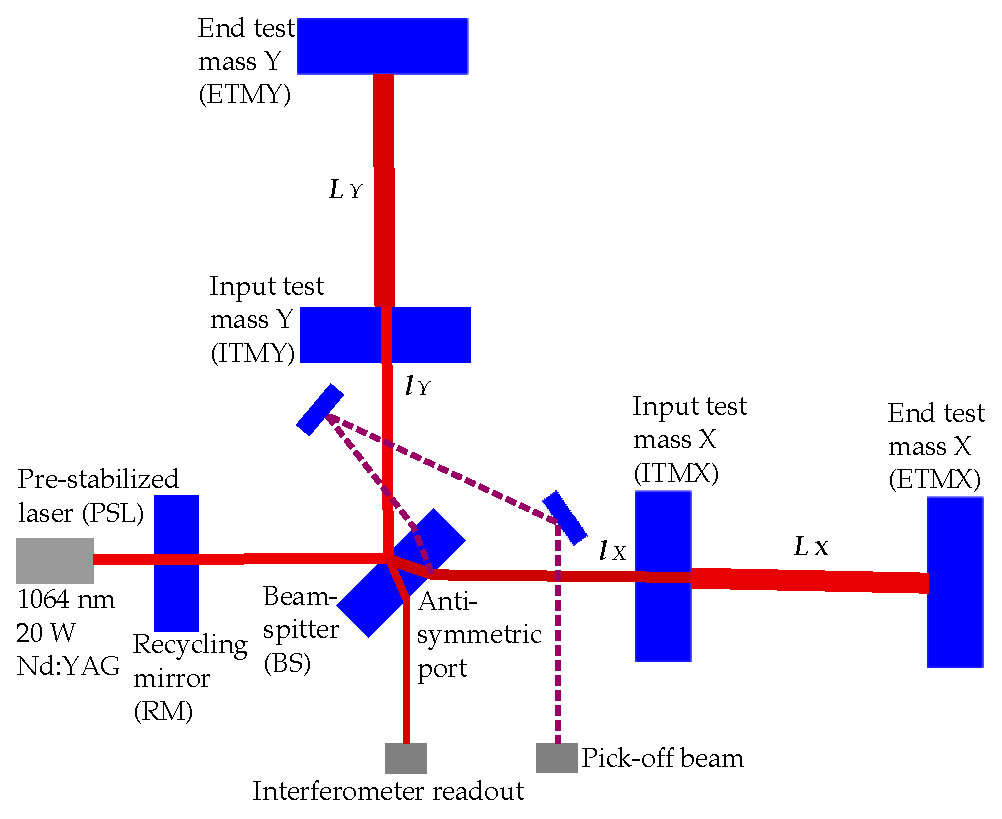
\includegraphics[height=135mm,width=150mm]{figure1.eps}
\caption{Gravitational wave strain $h(t)$ is derived from differential arm motion (DARM), read-out from a photodiode downstream of the antisymmetric port. An internal reflection off an anti-reflective coating, on either the beam-splitter (BS) or an input test mass (ITM), provides the Michelson (MICH) channel. The DARM readout channel predominantly measures the small change in different arm length, $\delta(L_-) \equiv \delta(L_y - L_x)$, while MICH measures that in the Michelson length $\delta(l_-) \equiv \delta(l_y - l_x)$. There is also a small coupling from $\delta(l_-)$ to the DARM channel. To a lesser extent, changes in the length of PRC, which is defined as $\delta(l_+) \equiv \delta(l_y + l_x)/2$ and is measured in quadrature demodulation with respect to the MICH pick-off, also add noise to DARM.}
\label{arms}
\end{center}
\end{figure}


        The value $\langle L_+\rangle$ is the nominal average arm length, about 4 km in LIGO. The distance function $z(\mathcal{X})$ indicates the distance\footnote{Note that $z(\textup{ITMY})$ is a function of both the ITMY and BS position}, along the optical path, from the laser to an optic $\mathcal{X}$; the variation $\delta$ denotes a change with respect to nominal value. DARM length is thus defined as $\delta(L_y - L_x)$ and MICH length as $\delta(l_y - l_x)$. In practice, DARM and MICH are the names given to the channels that predominantly measure those quantities. These channels are not so neatly delineated as the lengths. Unless stated otherwise, the terms DARM, MICH, PRC and CARM will refer to the measured channels, which are related to the lengths through calibration and are cross-contaminated (e.g., DARM = $L_{-} + \pi/(2 \mathcal{F}) l_{-}$, where $\mathcal{F}$ is cavity fineesse). The terms will not refer to the physical lengths in Equations~\ref{CARMdef} through~\ref{MICHdef}. 

        As Equation~\ref{DARMdef} and~\ref{MICHdef} imply and Figure~\ref{arms} illustrates, MICH noise makes the physical interpretation of DARM ambiguous. An arm cavity gain $r_{c}'/r_c \simeq 139/0.990$, where $r_c$ is the arm cavity reflectivity for the LIGO laser carrier frequency and $r_{c}'$ is the derivative of $r_c$ with respect to round trip phase~\cite{ReadoutGWA,BallmerThesis}, amplifies DARM motion for Initial and Enhanced LIGO. Where $\mathcal{F} \simeq 219$ is the cavity finesse, the gain is given by Equation~\ref{rcfactor}:

        \begin{eqnarray}
        \frac{r_{c}'}{r_c} = \frac{2 \mathcal{F}}{\pi} \simeq (139/0.990). \label{rcfactor}
        \end{eqnarray}

        \textit{A priori} MICH noise will leak into measurements of DARM with a transfer function equal to the inverse of Equation~\ref{rcfactor}~\cite{SiggFreq1997}. Empirically, coherence measurements confirm this coupling is the dominant part of the transfer function, but residuals suggest other effects exist. PRC is also indirectly correlated with DARM. These correlations are physical consequences of the interferometer design. 

In Enhanced LIGO, DARM is measured with a photodiode at the interferometer `dark' antisymmetric port of the beams-splitter. Independent photodiodes for MICH and PRC, used for feedback on their respective auxiliary length control servos, provide the witness channels for canceling cross-talk into DARM. The MICH and PRC photodiodes receive a beam from an internal reflection in the beam-splitter. This beam carries a radio-frequency modulation; one demodulation quadrature provides MICH, the other PRC.

        \subsection{Auxiliary noise coherence at sensitive frequencies}
        \label{aux_noise}

	 Cross-talk can be quantified with coherence, the Fourier frequency-dependent analog of statistical correlation. On a scale of 0 (none) to 1 (full), coherence represents the normalized fraction of power of a frequency bin in the spectrum of one channel that can be found in the same frequency bin in the spectrum of another channel. First, we must define the cross-power of a two time-series. Where $P_{xy}$ is cross-power spectral density as in Equation~\ref{Pyx}.

	Continuous and discrete definitions of cross-power $P$ follow; the operator $E$ denotes an expectation value, and $p$ and $q$ are discrete indices:
 
            \begin{eqnarray}
            P_{yx} (f) = \int_{-\infty}^{+\infty} \left(\int_{-\infty}^{+\infty} y^{*} (\tau) x(t+\tau) d \tau \right) e^{i 2 \pi f t} dt; \label{Pyx} \\
            P_{yx} (f, t) = \Sigma_{q=-t}^{t} R_{yx} (q) e^{-2 \pi i f q}, \label{Pyxext} \\
            R_{yx} (q) = E\left[ y_{p+q} x_p^* \right] \label{crossCovar}.
            \end{eqnarray}

Now we can describe how the coherence at a given frequency $f$ and time $t$~\cite{Boashash1990} is given by Equation~\ref{coherenceDef}. False positive rate for a coherence measure is governed by the probability that an observed coherence $C_{\textup{obs}}$ is greater than the actual coherence $C$. For a window factor $w$ (0.95 for a Hann window) and $N$ sample averages with Gaussian noise, the false positive rate is described in~\cite{MendellCohere2013} by Equation~\ref{CohereProb}
\begin{eqnarray}
C_{xy}(f, t) = \sqrt{\frac{\left| P_{xy}(f, t) \right|^2}{P_{xx}(f, t) P_{yy} (f, t)}}\label{coherenceDef}, \\
Prob\left( C_{\textup{obs}}^2 > C^2\right) = \left(1-C^2\right)^{w(N-1)} \label{CohereProb}
\end{eqnarray}

Uncorrelated channels have low coherence. The calibrated strain channel, Hoft\footnote{For clarity, we use Hoft to refer to the discrete-time calibrated strain data channel and $h(t)$ to refer to the corresponding physical strain.}, is measurably coherent with MICH and PRC, as seen in Figure~\ref{coherenceGraph}. MICH-DARM coherence, hence noise coupling, is sometimes as large as 0.1 in the 100 to 300 Hz band for the LIGO Hanford Observatory detector H1. Problematically, this is the most sensitive band for Initial and Enhanced LIGO. 


	Allen, Hua, and Ottewill~\cite{AllenHuaOttewill1999} first posited the filtering scheme that this paper employs. Where there is a strong correlation between a signal (target) channel and a noise (witness) channel, the noise can be partially cancelled if a witness-to-target transfer function, convolved with the witness, is applied to the measured target. Auxiliary MICH-PRC Subtraction (AMPS), a Matlab~\cite{Matlab2012a} pipeline, realizes this procedure.

AMPS fits an infinite impulse response (IIR) filter onto the most coherent frequency band of the witness-to-target transfer function. It processes LIGO Science Run 6 segment-by-segment, subdiving each segment into windows up to 1024 seconds in duration. S6 LIGO science segments exhibit MICH and PRC cross-talk primarily from 50 to 400 Hz. DARM is calibrated through a linear, frequency-dependent filter~\cite{LIGOCal2010} into the scientific channel Hoft. Since coherence and the technique of Allen, Hua, and Ottewill are both linear and transitive, AMPS has been designed to analyze Hoft data rather than analyzing DARM and duplicating the calibration filter.

Transfer function fitting is weighted toward 50-400 Hz by design in AMPS. Each transfer function for a given 1024 s of data is the average of 1024 independent ratios-of-Fourier-transforms (2047 Hann-windowed, 50\%-overlapping FFTs of 1 s samples of the 1024 s). Since the error in an FFT scales with the inverse square root of the number of averages, the relative accuracy for the transfer function is $\mathcal{O}\left(1024^{-1/2}\right)$. AMPS can proceed with less data, as little as 32 s, which yield $\mathcal{O}\left(32^{-1/2}\right)$ relative accuracy. Outside the 50-400 Hz band, the program deweights the fit to the transfer function and pre-processes it, suppressing it by factors of $(f/f_\textup{knee})^\alpha$, where $\alpha = 8$ at low frequencies and $-8$ at high, where $f_\textup{knee}$ was respectively 50 and 400 Hz. AMPS smooths and deweights (Figure~\ref{tfGraph}) known spectral peaks, including 60 Hz harmonics, the LIGO suspension violin modes, and calibration lines. Violin modes are internal resonances of the LIGO mirror suspensions caused by thermal noise; calibration lines are intentionally introduced narrow peaks in the spectrum used to help physically calibrate the interferometer in unit counts-to-length. De-weighting and pre-processsing, when carefully tuned, prevent AMPS from confusing the filter design with statistically insignificant transfer function data, which could introduce noise, as well as supporting faster and more accurate fit convergence with fewer free parameters.

        \subsection{Estimating filters}
        \label{filter_est}

	Parameters for the transfer function are determined by Vectfit, developed by Gustavsen et al.~\cite{Deschrijver2008,Gustavsen2006,Gustavsen1999}. Vectfit iteratively fits a state-space model to the numerically-estimated transfer function. AMPS calls Vectfit on one channel at a time, as will be discussed in Section~\ref{out-of-loop}. Each iteration of Vectfit uses pole-shifting to optimize a state-space model of the transfer function according to a least-squares fit. Empirically, convergence on a model was achieved after about five iterations on S6 data; we chose fifteen iterations for a safety margin, enforcing stable poles on the complex left half-plane. After sufficient iterations, the transfer function model (for AMPS, 32nd order) is extracted. 

Before applying the filter, different representations of the transfer function model are used to validate key parameters. Zero-pole-gain (ZPK) format is used to trim out-of-band zeroes and poles and multiply by a 2nd order Butterworth low-pass filter just below the Nyquist frequency of 8192 Hz, placing poles at 7 kHz to ensure causality. An overall scale factor is applied to the low-pass to keep the filter gain at 150 Hz the same value as the regression in Vectfit. AMPS converts the ZPK model to second-order-section (SOS) digital filter format for numerical stability. Instead of the inverse Fourier transform of Equation~\ref{gcf}, this SOS model is converted from continuous time (or $s$-domain) to discrete time (or $z$-domain). Finally, using the discrete-time SOS representation, the IIR filter is applied to its respective witness channel. The estimated true Hoft target equals the original Hoft measurement minus the filtered witness channels. 

This procedure makes two assumptions. It assumes that the dominant coupling from each witness channel into Hoft is linear. Further, it assumes that 2nd order coupling, from one witness channel into the other and subsequently into Hoft, is negligible. Expectations and spot-check measurements confirm that these assumptions are justified approximations.  

	Equations~\ref{Txy} through~\ref{hatsf} capture this method. It is analogous to frequency-domain principal component analysis (PCA) using Gram-Schmidt orthogonalization. Allen, Hua, and Ottewill established the mathematical theory, using superscript $^{(b)}$ to indicate a frequency band that we denote as domain $(f)$. Their Equations~7, 8, and 11 correspond, respectively, to Equations~\ref{Pyx},~\ref{hatsf} and~\ref{Txy} here.

A transfer function $T$ can be expressed as the cross-power ratio of arbitrary channels $x$ and $y$:

            \begin{eqnarray}
            T_{xy} (f) = \frac{P_{yx}(f)}{P_{xx}(f)}. \label{Txy}
            \end{eqnarray}

\noindent The estimated feedforward filter $g$ can be viewed as an inverse Fourier transform $\mathcal{F}^{-1}$, decoupling signal (target, subscript $s$) from noise (witness, subscript $n$):
            \begin{eqnarray}
            g(t) = \mathcal{F}^{-1} \left( \textup{fit} \left[ T_{sn} (f) \right] \right) \label{gcf}.
            \end{eqnarray}
\noindent Finally, the post-filtering signal (target) $\hat{s}$ can be written in terms of convolution (the $\times$ sign) with $\gamma$, the transfer function coupling noise (witness) into signal (target), $s$ pre-filter signal, $n$ noise, and with channels indexed by $j$ and curly brackets indicating an observable quantity: 
            \begin{eqnarray}
            \hat{s} (t) = \left\{ s + \Sigma_j \left(\gamma_j \times n_j\right)\right\} (t) - \Sigma_j \left(g_{j} (t) \times \left\{ n_{j} \right\} (t)\right) \label{hatsf}.
            \end{eqnarray}


Blind application of this method could theoretically produce unwarranted noise reduction. Application of this paper's method to uncorrelated channels would lead to unwarranted noise reduction by an analytic factor of $(1 - 1/F)$~\cite{AllenHuaOttewill1999}, where F is the number of bins in a fitted frequency span, or, in time-domain, the number of averages. Given 1-s windowing with 50\%-overlap on 1024 s, $F = 2047$, for an unwarranted noise reduction of about 0.05\%. The ideal of 1024-s windows is not always achievable with LIGO duty cycles. In these cases, AMPS incorporates some filters estimated on as little as 32 s of data, for which the unwarranted reduction would be 3\%, but only when these filters are averaged together with longer-duration (512 s or greater) filters. No isolated filter is estimated on less than 60 s of data, which could yield an uncorrelated noise reduction of 1.5\%. Allen, Hua, and Ottewill clarify that subtraction is tenable so long as covariance (in frequency-domain, coherence) is present at a statistically significant level. They set a benchmark of an order-of-magnitude above the magnitude-square covariance expectation value of $1/F$. Since the AMPS pipeline emphasize fits in regions where the coherence is greater than 3\%, and often 10\% or more, it usually satisfies their criterion.


\begin{figure}
\begin{center}
\includegraphics[height=80mm, width=75mm]{figure2a.eps}
\includegraphics[height=80mm, width=75mm]{figure2b.eps}
\caption{Sample coherence measurements between Hoft and auxiliary control channels for LIGO Hanford Observatory, H1: 2010 March 21. Hoft-to-MICH coherence on left, Hoft-to-PRC coherence on right. Statistically significant coherence justifies fitting; in frequency bands, about 80 to 400 Hz, where coherence rose above background levels, the transfer function fit was weighted more heavily. Units of coherence spectral density (Hz$^{-1/2}$) vs frequency (Hz).}
\label{coherenceGraph}
\end{center}
\end{figure}
\begin{figure}
\begin{center}
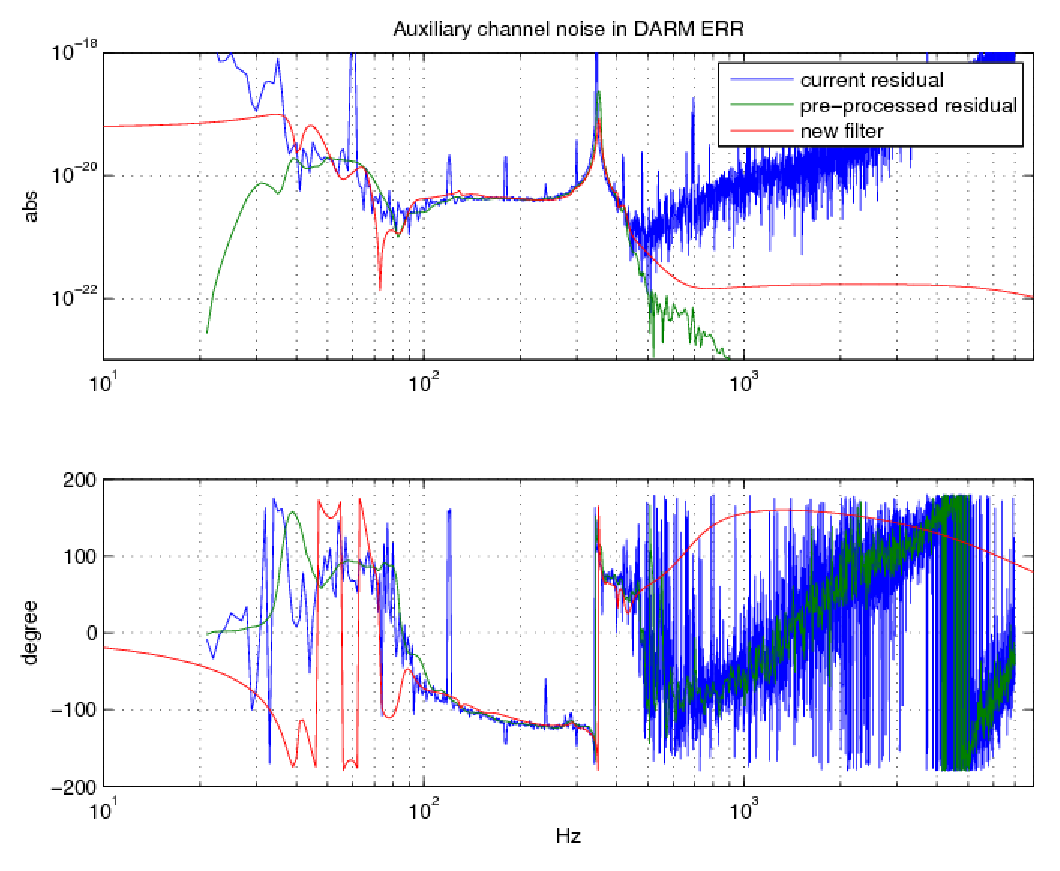
\includegraphics[height=100mm, width=75mm]{figure3a.eps}
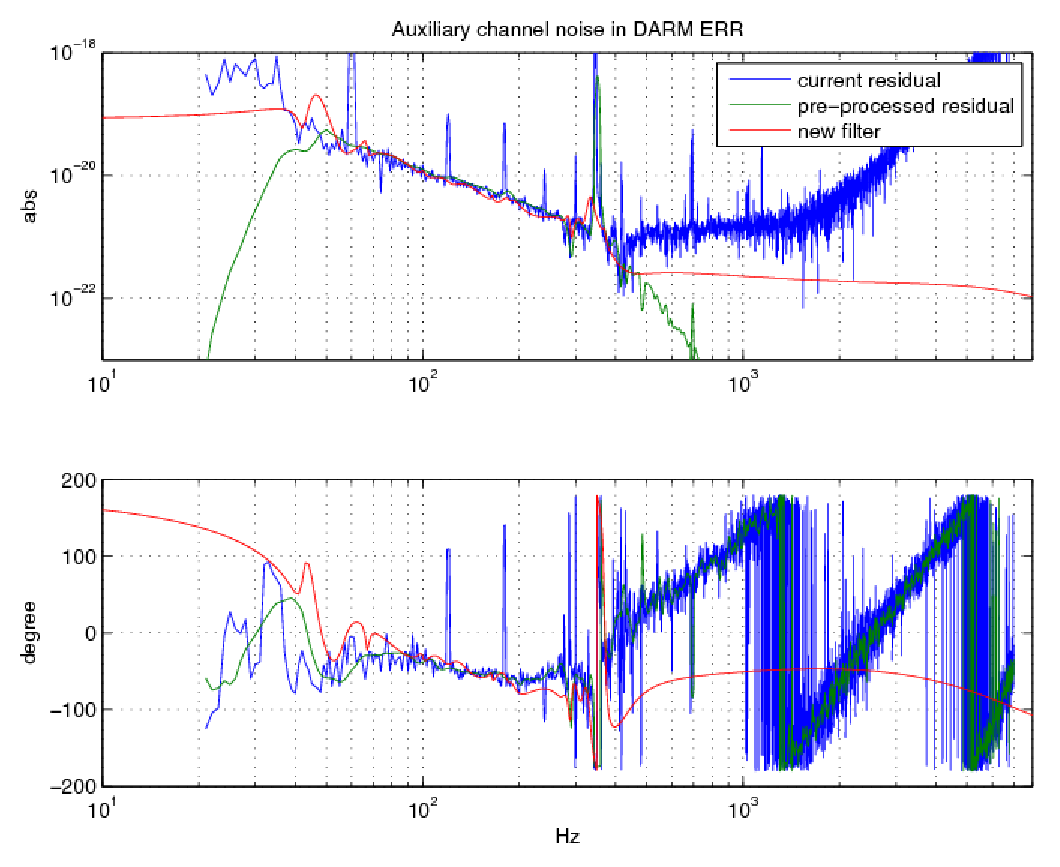
\includegraphics[height=100mm, width=75mm]{figure3b.eps}
\caption{Sample transfer function measurements (amplitude and phase) from LIGO Hanford Observatory, H1: 2010 March 21; MICH on left, PRC on right. Transfer function fit in coherent band -- note the difference between raw data residual and the `pre-processed residual', which has been smoothed and weighted to emphasize known-coherent bands. Units of amplitude spectral density (Hz$^{-1/2}$) and phase (degrees) vs frequency (Hz).}
\label{tfGraph}
\end{center}
\end{figure}
\begin{figure}
\begin{center}
\includegraphics[height=100mm, width=75mm]{figure4a.eps}
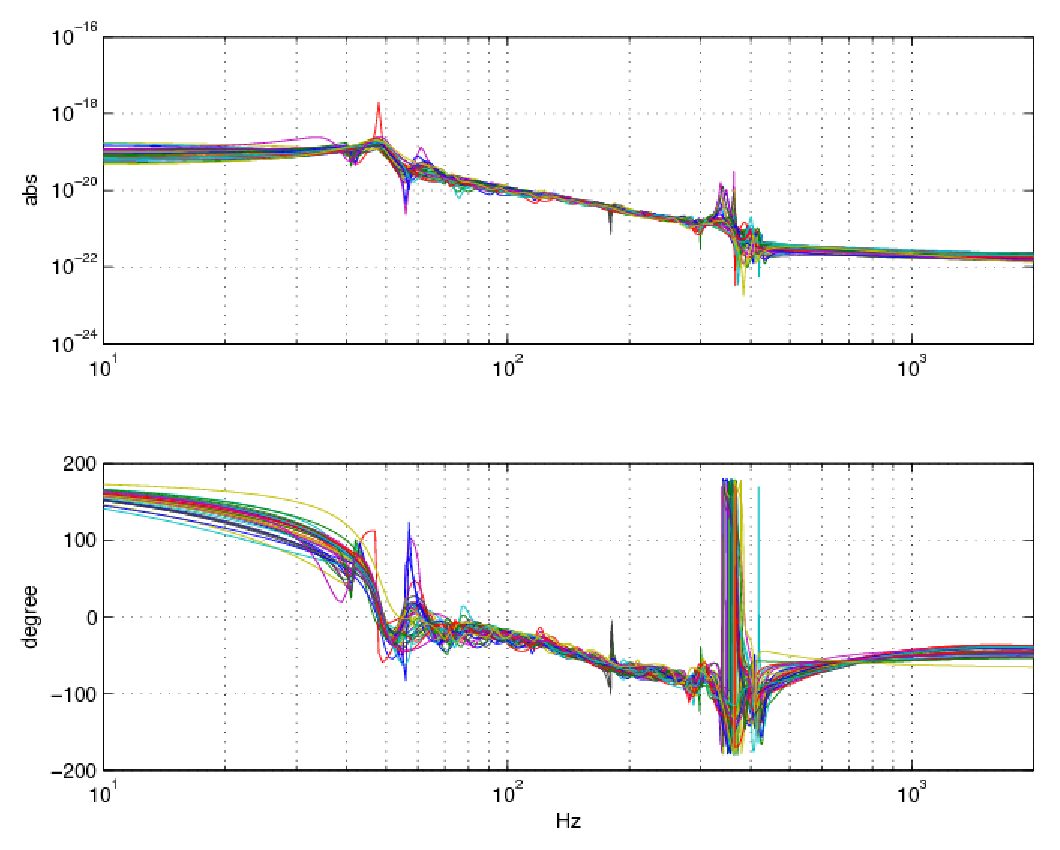
\includegraphics[height=100mm, width=75mm]{figure4b.eps}
\caption{Sample Bode plots of fitted ZPK filter functions (amplitude and phase) for multiple 1024 s windows in a science segment, at LIGO Hanford Observatory, H1: 2010 March 21; MICH on left, PRC on right. The similarity in the high-coherence, 80 to 400 Hz band leads us to conclude that the filter design is fairly stable throughout a science segment. Units of amplitude spectral density (Hz$^{-1/2}$) and phase (degrees) vs frequency (Hz).}
\label{BodePlots}
\end{center}
\end{figure}
\begin{figure}
\begin{center}
\includegraphics[height=80mm, width=75mm]{figure5a.eps}
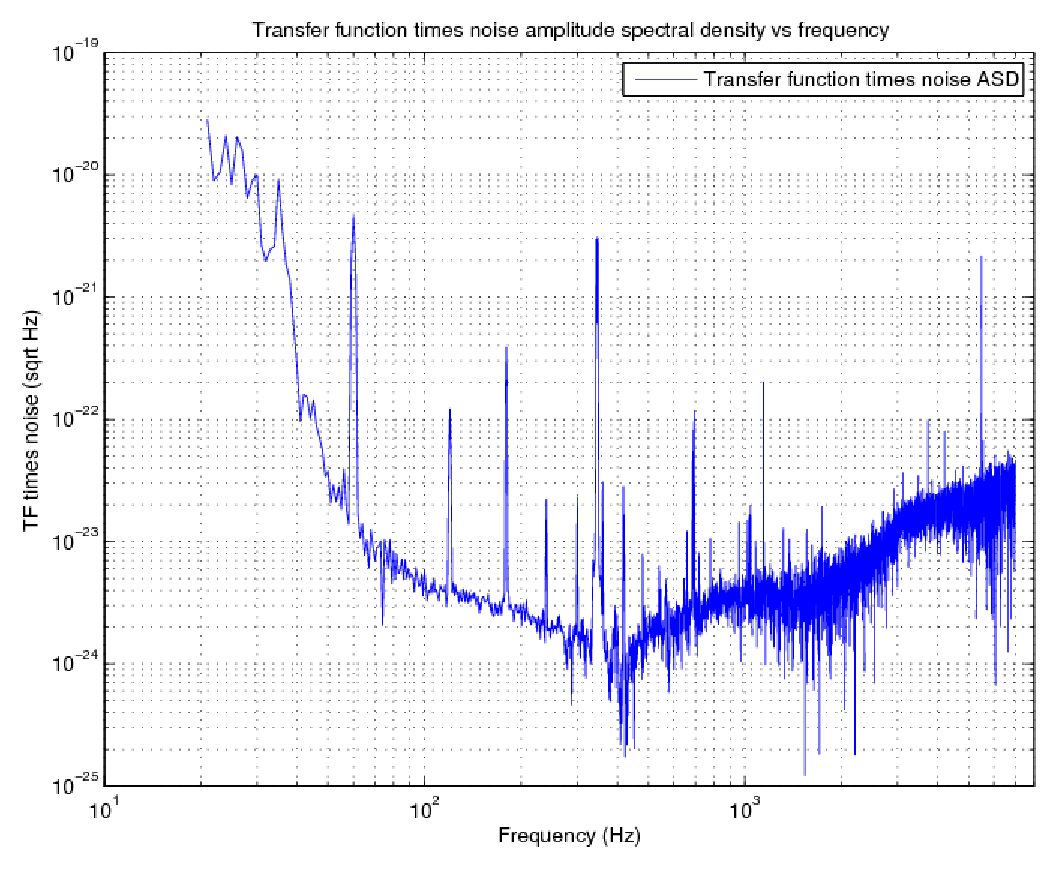
\includegraphics[height=80mm, width=75mm]{figure5b.eps}
\caption{Sample subtracted spectra for one window, representing the applied feedforward corrections for each channel during that window, at LIGO Hanford Observatory, H1: 2010 March 21; MICH on left, PRC on right. Units of amplitude spectral density (Hz$^{-1/2}$) vs frequency (Hz).}
\label{subtractedSpectrum}
\end{center}
\end{figure}

As described in Section~\ref{filter_fitting-out-of-loop}, the filters calculated for each 1024-s window are blended to generate the estimated target for a whole science segment. Figure~\ref{BodePlots} illustrates the short-term consistency of transfer functions during a few-hour science segment, presenting a Bode plot of Hoft-MICH transfer function fits for consecutive windows from 2010 March 21 at LIGO Hanford Observatory (magnitude, top and phase, bottom vs frequency [Hz]). These transfer functions varied more markedly over longer timescales of months, reflected in the fluctuating amount of improvement seen in Figures~\ref{typicalInspiralGraph} and~\ref{bestInspiralGraph} (covering $4\times10^6$ seconds of data). Figure~\ref{subtractedSpectrum} presents a sample subtraction for one 1024-s window. These figures show that AMPS successfully, efficiently realizes the intent of Allen, Hua, and Ottewill on operational data for a kilometer-scale gravitational wave interferometer.

Section~\ref{prior_programs} sets this method in context, Section~\ref{safeguards} discusses safeguards and vetos, and Section~\ref{out-of-loop} discusses the details of implementation and verification.

    \section{Feedforward in-loop and alternative program methods}
    \label{prior_programs}
   
        During LIGO running, real-time feedforward subtraction for MICH and PRC noise must meet operational constraints. Existing manually designed filters have certain tradeoffs compared to Vectfit-designed filtering; new methods, such as the Wiener filtering now being considered for seismic and gravity-gradient cancellation, are also possible~\cite{Driggers2012ActiveNoise}.
        
        \subsection{Manually designed rational filtering in-loop}
        \label{manual_design}

            Manual designs of feedforward functions prove time-consuming. Transfer functions can be manually fit using the LIGO Foton filtering system~\cite{Sigg2005} or a comparable filter design tool. Several additional transfer function measurements are needed for a filter deployed in-loop, in order to compensate for servo loop gain and actuation functions. Manual design is not an efficient alternative to algorithmic transfer function design: it is labor-intensive to repeat regularly, and the results of our run over S6 suggest that filter redesign should be performed often.

	While labor-intensive, manual-designed rational filtering of MICH and PRC in-loop provides a necessary part of LIGO servo controls. The auxiliary control channels intrinsically introduce `self-inflicted' noise into the DARM channel, and without real-time correction, the performance of its science runs would be much worse than design sensitivity. The majority of MICH/PRC subtraction comes from this real-time correction; AMPS as used on S6 data is a comparatively small perturbation, one to two orders of magnitude smaller.

        \subsection{Vector-fitted filter functions}
        \label{vectfit}

            Algorithmic fitters such as Vectfit allow automated design of transfer functions. Because it is automated, the filter can be made adaptive by periodic re-design. Since the dynamic range in magnitude for LIGO length control channels, and consequently transfer functions, can vary over tens of orders of magnitude, one must take care to weight and pre-process data, especially when operating in the most sensitive band from 100 to 300 Hz. Although not the only possibility, Vectfit, applied to a single witness-target pair, is straightforward. Vectfit iterates a rough \textit{prior} set of pole locations, translating it across the complex plane according to a least-squares fit of the rational function onto transfer function data. About five iterations achieve good convergence. AMPS employs Vectfit's report on cumulative goodness-of-fit, root-mean-square (RMS) error, as a statistic to decide whether to reject Vectfit's filter regression. Using this statistic allows AMPS to isolate a failure in regression to one channel. From empirical studies, RMS error above $1\times 10^{-18}$ indicates a poor fit, where the fit residual of frequency bin $i$ is $\Delta_i$ ($i \in [1,...,N]$), and RMS error $\sigma$ is defined by Equation~\ref{RMSerrorDefinition}:

\begin{eqnarray}
\sigma = \frac{\sqrt{\Sigma_{i=1}^N \left| \Delta_i \right|^2}}{\sqrt{N}}\label{RMSerrorDefinition}.
\end{eqnarray}

        \subsection{Wiener filters}
        \label{wiener_filters}

            Wiener filtering~\cite{Wiener1949} searches for an optimal filter of a particular kind: it minimizes the squared error of the residual. However, the error is over the entire spectrum. Coherence at low-frequencies in MICH-PRC applications is low, but a Wiener filter by default will fit their high-power at the expense of lower-power, higher frequency bands. That fit would be statistical unsubstantiated and counterproductive, if calculated for the entire spectrum at once. Filters that intentionally focus on bands with high RMS power, such as seismic and gravity gradient noise, can use Wiener filtering without difficulties. Several methods can be used to treat this challenge for more general cases.  Noise whitening~\cite{Driggers2012NN,DeRosa2012FF} can use frequency-weighted cost functions to limit noise injection from out-of-band. Data over the dynamic range of LIGO's bucket may also be addressed by band-passing the spectrum into sub-spectra. Evaluating the error over sub-spectra could circumvent contamination from the high spectral power present at low-frequencies.  Transforms that break the spectrum up into many bands, such as wavelet transforms~\cite{KlimenkoSite}, seem promising.  

At the Caltech 40m prototype gravitational wave antenna, Wiener filtering has been used to prototype measures for dealing with Newtonian and seismic noise in advanced interferometers~\cite{Driggers2012ActiveNoise}. Wiener filtering is theoretically the optimal kind of filtering for balancing the gain from feedforward correction against the harm done when witness channels are themselves noisy. In the case of MICH and PRC, the channels are relatively good witnesses, but in other situations, Wiener filtering might provide superior performance. There is no reason to think that Wiener filtering would not provide MICH and PRC feedforward subtraction equal to what is obtained using a numerically determined transfer function (fit to IIR form using Vectifit). The latter was computationally-compelling for the AMPS pipeline. 


        \subsection{Prospects for almost-real-time filtering}
        \label{real-time}
      
            Auxiliary MICH-PRC Subtraction (AMPS) code, as presented by this paper, is designed to provide out-of-loop, post-facto Vectfit feedforward subtraction that meets criteria for statistically soundness and accuracy. The software must also be efficient. Auxiliary MICH-PRC Subtraction code runs a few times faster than real-time on 2013 hardware whilst conducting extensive tests and safeguards, documented in Section~\ref{safeguards}. Unfortunately, failing the veto triggers extends the time-to-completion. Long program time is acceptable for a side-channel generating in data when a reference Hoft, measuring $h(t)$, already exists. This arrangement is not ideal for in-loop, real-time production of $h(t)$. Even if the vetos are not triggered, the maximum time delay between a sample and its final, corrected form is the time at which the filter is generated, up to a window (1024-s) in the future. This lag is undesirable for electromagnetic follow-up, part of the multi-messenger astronomy~\cite{Swift2012,Antares2013} desired for Advanced LIGO. 

A modified system that could operate in almost-real-time batches, refreshing periodically with prior data from the same science segment, might be useful for countering upconversion and other non-linear features of cross-coupling. One method for true real-time use of an AMPS-derived pipeline would be to output filters periodically for use in upcoming real-time data, that is, to use the windowing system to designate training sets. These features, however, are not yet implemented.

\section{Safeguard and veto methods}
\label{safeguards}

    \subsection{Runtime safeguards}
    \label{runtimeSafeguards}

Gravitational wave strain, $h(t)$, is the most important data channel for LIGO; the AMPS pipeline takes several measures to ensure its integrity. Post-facto adjustments are unusual; when individual LIGO searches process $h(t)$, they typically do not apply any correction based on auxiliary channel data. Such corrections have been the province of real-time servos. Real-time servo techniques work well, and if a problem is detected, it can often be fixed within a short commissioning break. Sometimes, the problem is an ephemeral `glitch' with no straightforward solution. Should time and resources for an immediate fix not be available, it is advantageous to have methods for revisiting the data and attempting a correction after the fact. AMPS is useful for providing this kind of correction, and by improving $h(t)$ itself -- rather than pre-processing data for a particular search -- it potentially benefits all LIGO analyses.

Given the new approach here, AMPS verifies data integrity through several safeguards and vetoes against known and possible issues. These issues include making data worse, offsetting and incorrectly time-stamping the data, incorrectly subtracting $h(t)$ from itself, and introducing Fourier transform windowing artifacts.

After filtering each window, AMPS calculates its amplitude spectral density in Matlab using Welch's method (\texttt{pwelch} in Matlab)~\cite{Matlab2012a,Welch1967}, which enables calculating inspiral range $\mathcal{R}$, an astrophysical measure of performance~\cite{FinnInspiral1993} and quantifying  the change in spectrum. The window's filtered data is used, if post-filter $\mathcal{R}$ is at least 99.9\% of unfiltered $\mathcal{R}$, and if none of the 40 points in a `comb' (each point being 5/16 Hz wide) of quiet bands is noisier in AMPS $h(t)$ value than 1.2 times uncorrected, Hoft $h(t)$. If the window fails this test, it is passed back through the windowing method and combined with baseline, unfiltered LIGO data from the same window until it passed the veto. This process allows for progressive diminuation of the influence of any abrupt non-stationary features in the transfer function that may be causing the test to fail. Eight such `re-normalizing' cycles are tried -- if those fail, it then writes what it has and proceeds to the next segment. Empirically, it is found that these criteria ensure that almost all AMPS data is better, on average, than Hoft raw data, because it selects the better of either baseline or filtered data.

    \subsection{Post-processing safeguards}
    \label{postprocessingSafeguards}

Besides imposing these runtime safeguards, the AMPS project computes diagnostics to check whether calibration lines (Figure~\ref{calLineTest}) are diminished -- which would indicate that AMPS was incorrectly subtracting $h(t)$ from the Hoft channel. It also checks whether injections (Figures~\ref{timeDomainInjection} and \ref{crossCorrelationGraph}) are recovered at the correct times. These injection studies examine compact binary coalescence and sine-Gaussian hardware injections~\cite{LIGOBurst2012} for GPS seconds $931.0 \times 10^6$ (2009 July 07) to $932.8 \times 10^6$ (2009 July 28) and produced basic time-domain plots and cross-correlations. In addition, to verify that the ability to observe compact binary coalescences is not decreased by AMPS, we calculate the matched-filter signal-to-noise ratio of each of the compact binary coalescence hardware injections in the S6 data. This is done by filtering each hardware injection against the compact binary coalescence waveform that was used when the hardware injection was performed. The matched filter signal-to-noise ratio is directly proportional to the distance at which such a signal can be observed, and therefore also to the overall sensitivity of the instrument to signals of that type~\cite{Findchirp2012,PetersMatthews1963}. These tests affirmed the result that feedforward data contains recoverable (and slightly higher signal-to-noise ratio) injections.

Calibration line studies seek to answer two questions: whether feedforward distorts the signal and whether it adds noise. The latter question is answered in the affirmative if we find windowing artifacts, such as spectral combs with spacing of 1/1024 or 1/512 Hz, that might be generated around a prominent line. In post-processing, so-called `Short Fourier Transforms' (SFTs) were made with a finer frequency resolution (1/1800 Hz, by taking 1800 s stretches of data) from the generated AMPS time series. These SFTs are short in the sense of being shorter than the duration of a (potentially year-long) science run, and the 1800 s duration was chosen because it is the standard for LIGO continuous wave searches. The fine frequency resolution of SFTs should have made any artifacts visible. Post-processing tools saw no new combs in our 1800-s, 50\%-overlapping Hann-windowed SFTs before/after comparison of  approximately $10^6$ s of H1 science time between GPS times $931.0 \times 10^6$ (2009 July 07) and $932.8 \times 10^6$ (2009 July 28). The 393.1 Hz calibration line\footnote{Strictly speaking, the line visible in Hoft is a residual artifact from the imperfect cancellation of control and error signals used in the construction of Hoft $\propto h(t)$ from the DARM error and DARM control signals. The accidental nature of the line does not affect our analysis, because neither MICH nor PRC affect the line.} exhibited no noticeable comb artifacts. The signal-distortion question is answered by taking the mean of the three 1/1800 bins in the range of [393.1 - 1/1800, 393.1 + 1/1800] Hz: for the $10^6$ s of H1 science time analyzed, the before-feedforward mean was $1.3082 \times 10^{-21} (\textup{Hz})^{-1/2}$, whereas afterward it was $1.3128 \times 10^{-21} (\textup{Hz})^{-1/2}$. Feedforward made the calibration line region noisier by $4.6 \times 10^{-24} (\textup{Hz})^{-1/2}$ or 0.35\%. Evaluating the three bins around the calibration line helps to account for possible spectral leakage, since the central line is much larger than its neighbors.  

We conclude that we are not subtracting Hoft/DARM from itself. The additional noise is perhaps due to the low weighting of the AMPS transfer function fit at the 393.1 Hz line: that part of the spectrum is not tightly fit, because it could bias more sensitive parts of the spectrum.

\begin{figure}
\begin{center}
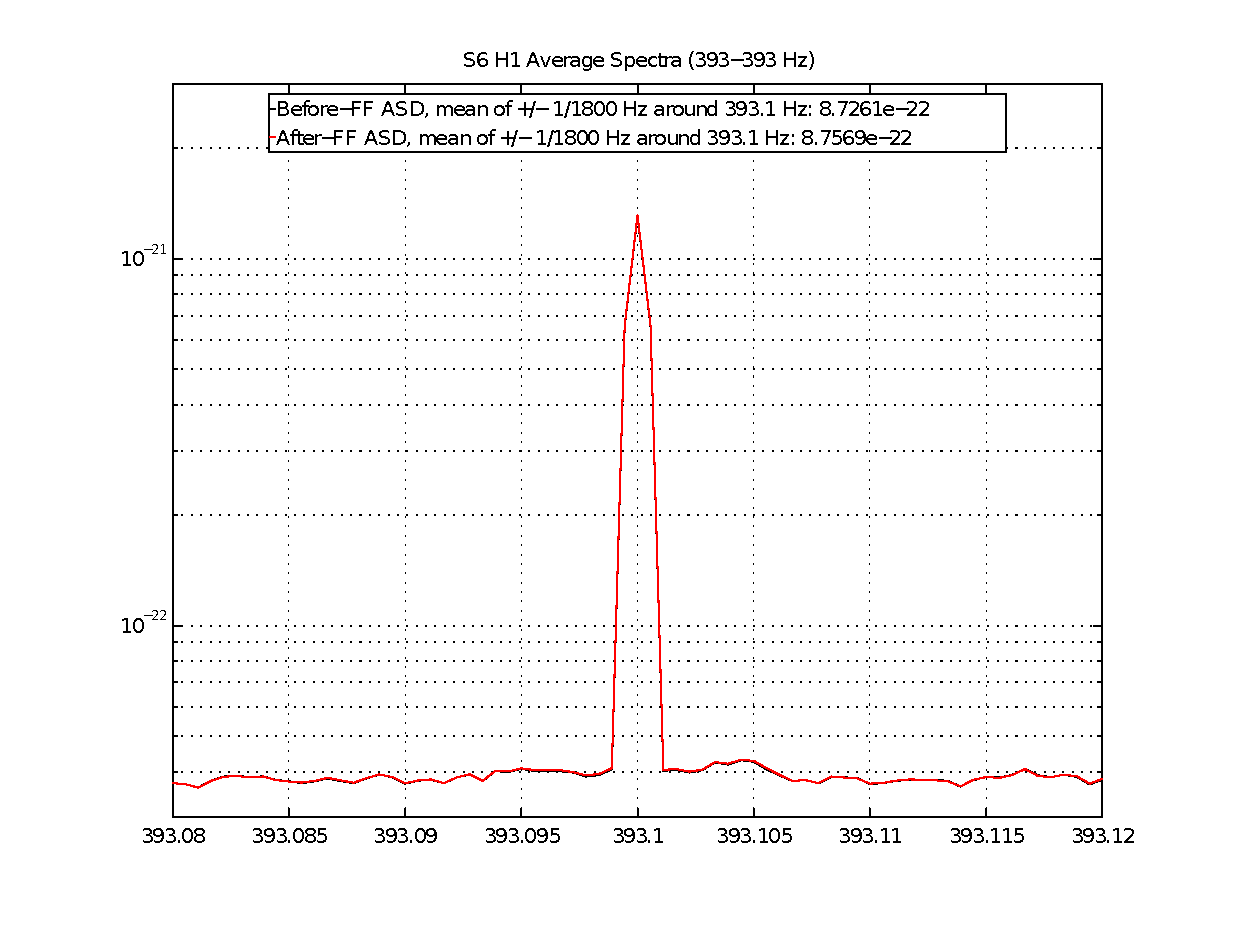
\includegraphics[height=75mm, width=150mm]{figure6.eps}
\caption{Calibration line test: before-feedforward mean of the 393.1 Hz line and two neighboring FFT bins was $1.3082 \times 10^{-21}$, after was $1.3128 \times 10^{-21}$. Feedforward made the calibration line region noisier by $4.6 \times 10^{-24}$ or 0.35\%, suggesting that we correctly apply Hann-windowed feedforward without subtracting true $h(t)$. Moreover, no spectral line combs are observed to either side of the calibration line peak at 393.1 Hz, indicating that the method does not introduce windowing artifacts.}
\label{calLineTest}
\end{center}
\end{figure}

\begin{figure}
\begin{center}
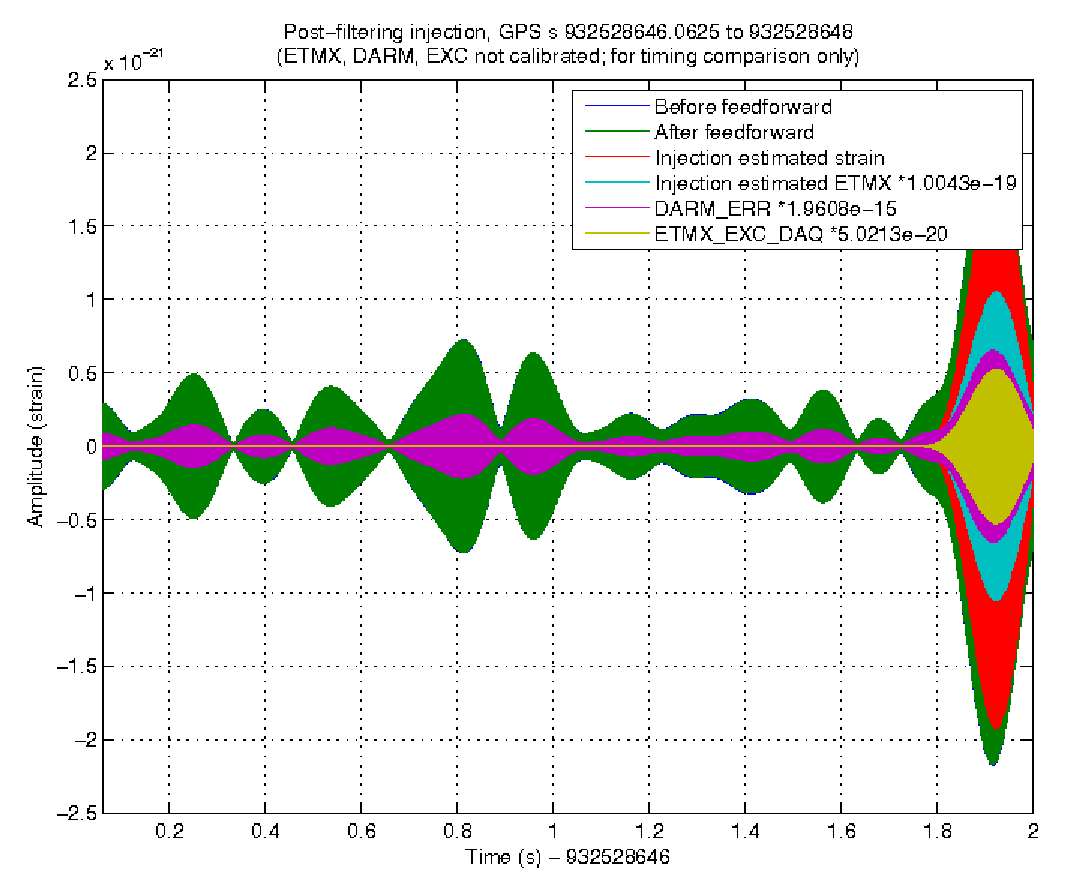
\includegraphics[height=75mm, width=150mm]{figure7.eps}
\caption{Time-domain plot of diagnostic channels from a burst injection: the simultaneous envelope increase after 1.8 s indicates that the burst injection is correctly time-stamped in the new data. `Before feedforward' and `after feedforward' traces occult each other in the graph, because they are almost identical. `Before feedforward' is Hoft data; `after feedforward` is AMPS data with feedforward subtraction. `Injection estimated strain' is the digital injection as intended to be introduced into strain, but the actual injection is made on the end test mass X (ETMX), so the calibrated `Injection estimated ETMX' is also displayed, along with the raw `DARM' differential arm channel and raw `ETMX' channel.}
\label{timeDomainInjection}
\end{center}
\end{figure}

\begin{figure}
\begin{center}
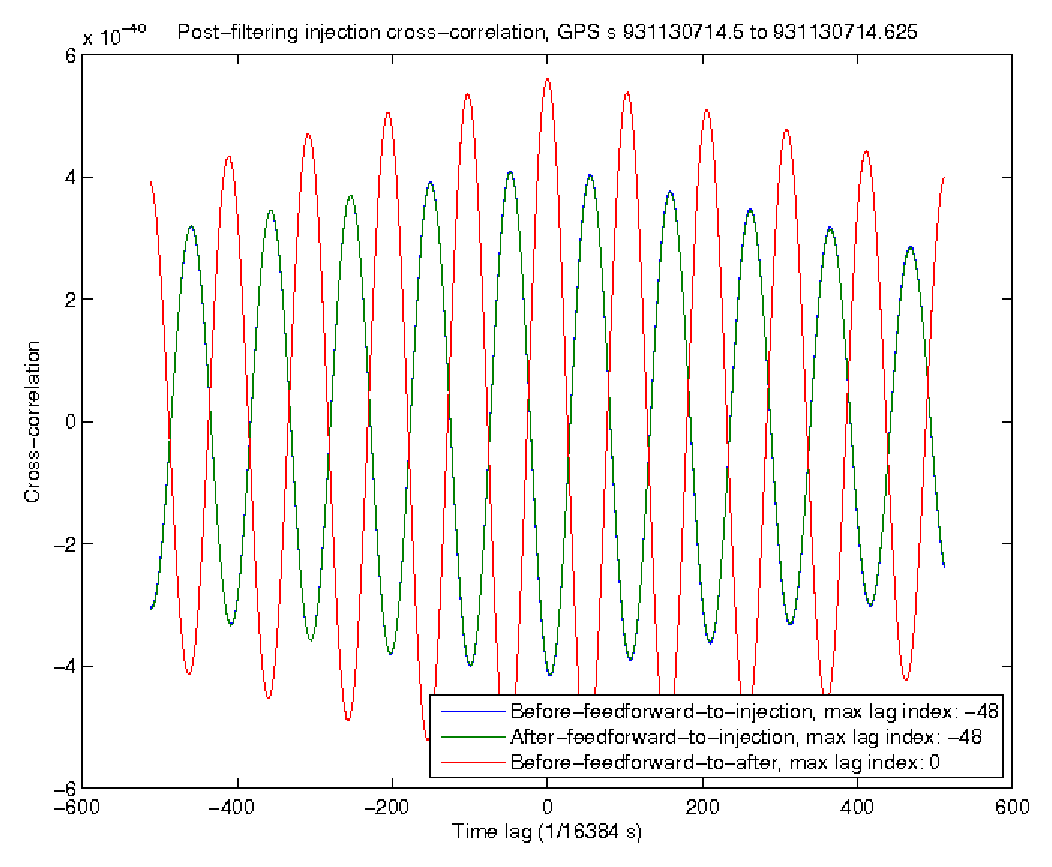
\includegraphics[height=75mm, width=150mm]{figure8.eps}
\caption{Cross-correlation pairwise between pre-, post-feedforward, and injection data: the extrema and zero-crossings match.  Note both before-feedforward (blue) and after-feedforward (green) strain traces are almost identical and therefore overlap. The strains appear inverted, but in the same way, due to a sign error in the hardware injections at this time.}
\label{crossCorrelationGraph}
\end{center}
\end{figure}

        From the nearly equal height of the calibration line before and after and the identical lag of the before and after feedforward strains with respect to the injections, we have confidence that AMPS is not subtracting $h(t)$ from itself, and that it is not shifting the samples in time.

    \section{Feedforward results and discussion: MICH and PRC channels}
    \label{out-of-loop}

\begin{figure}
\begin{center}
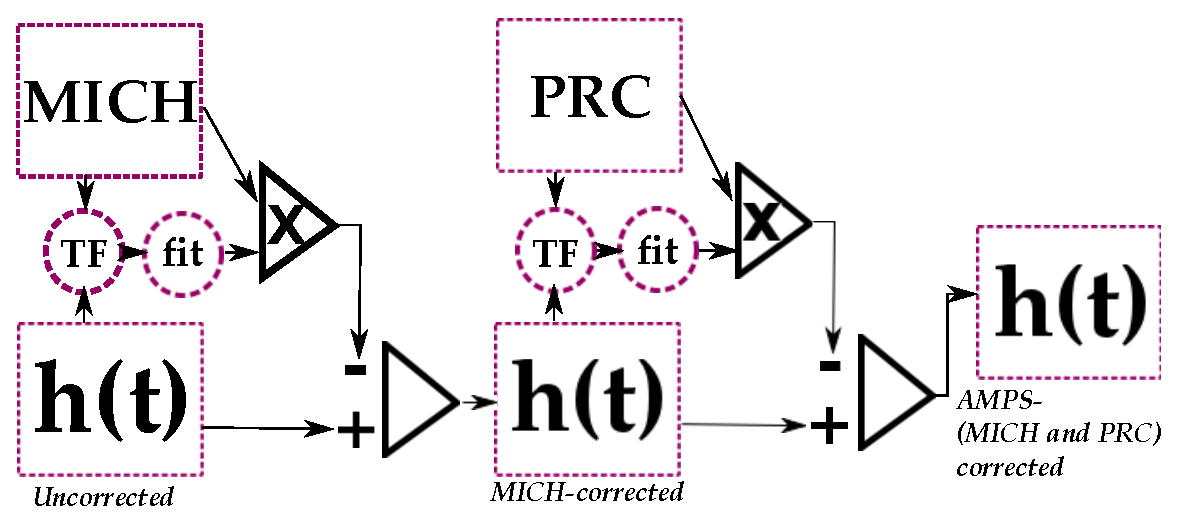
\includegraphics[height=100mm,width=150mm]{figure9.eps}
\caption{Feedforward subtraction pipeline to read in Hoft (calibrated DARM), MICH, PRC, and write out AMPS (clean calibrated DARM). Data flows schematically from left to right; the MICH-Hoft stage output is used as input for the PRC-Hoft stage, then AMPS data frames are finally written. Code can be found in the LIGO Matapps SVN: \texttt{matapps/packages/detchar/AMPS/trunk/aletheia.m}}
\label{pipelineGraph}
\end{center}
\end{figure}    

Realizing a post-facto, linear filtering engine, AMPS includes \texttt{aletheia.m}, a Matlab function in the Auxiliary MICH-PRC Subtraction package that fits and applies a filter to either MICH or PRC (specified by an argument). The fit occurs in the frequency-domain. The filter is applied in the time domain. From a high-level perspective, it is a system for reading in Hoft frames, correcting them with MICH and PRC frames, and writing AMPS data frames, accompanied by data quality and state vector channels, and producing diagnostic graphs. The pipeline is shown in Figure~\ref{pipelineGraph}. 


        \subsection{Filter fitting across science segments}
        \label{filter_fitting-out-of-loop}

So as to run efficiently on a LIGO computing cluster, the AMPS pipeline processes one filtering job per science segment. LIGO science segments range in duration from seconds to days, with the median segment typically lasting hours. During each segment, the interferometer is continuously locked, meaning it is held fixed on one interferometric fringe, by servo controlling all degrees of freedom so that they are stationary. If lock is lost, the segment ends. Serious noise degradations can also define the end of a segment. Each segment is managed by the main AMPS program, \texttt{eleutheria.m}. This program windows the segment, with windows up to 1024 s long, passes them to the filtering function and merges them smoothly together using 50\%-overlapping Hann windowing. Windowing is idempotent for raw Hoft; the only difference from window to window is the correction added to Hoft. The first 512 s are entirely driven by the first window; every 512 s thereafter, a new window is introduced, as in Figure~\ref{windowingScience}.


Using Equation~\ref{hatsf} with filters $g$, target $S = \left\{ s + \Sigma_j \left(\gamma_j \times n_j\right)\right\}$ and witness $N_j = \left\{ n_{j} \right\}$, we can evaluate  $\hat{s} (t)$. Since the filters for different channels are calculated in series, with transfer functions $T$, Equation~\ref{hatexpand} has $g_1 \sim T_{S,N_1}$ but $g_2 \sim T_{\left( S-g_1 \times N_1 \right),N_2}$. In AMPS, $S$, $N_1$ and $N_2$ are respectively the Hoft, MICH and PRC channels.

            \begin{eqnarray}
            \hat{s} (t) &=& S (t) - \Sigma_j \left(g_{j} (t) \times N (t)\right) \label{hatexpand}, \\
		&=& S (t) - g_1 (t) \times N_1 (t) - g_2 (t) \times N_2 (t) \label{hatexpanded},\\
&\sim& S (t) - \mathcal{F}^{-1} \textup{fit}\left[ T_{S,N_1} \right] \times N_1 (t) - \mathcal{F}^{-1} \textup{fit}\left[T_{\left( S-g_1 \times N_1 \right),N_2} \right] \times N_2 (t).
            \end{eqnarray} 
		

	Since $N_1(t)$ and $N_2(t)$ are added linearly to $S(t)$, we can analyze them independently. 
For clarity, analyze only the first two terms of Equation~\ref{hatexpanded} and take $N(t) = N_1(t)$. Let $g_{A}$ and $g_{B}$ be the earlier and later filters for $N(t)$ being time-domain merged in a Hann-window; they are respectively calculated from overlapping data sets $[S_A, N_A]$ and $[S_B, N_B]$. The sets are sample-for-sample identical at a given time $t$, so $S(t)=S_A(t) = S_B(t)$, $N(t)=N_A(t) = N_B(t)$. AMPS merges data streams $\hat{s}_A$ and $\hat{s}_B$ over the window $\tau = 1024$ s to effect the windowing, per Equation~\ref{windowexpand}: 

	\begin{eqnarray}
        \hat{s} (t) &=& \frac{\hat{s}_A (t)}{2} \left[1 - \cos \frac{2 \pi (t+\frac{\tau}{2})}{\tau} \right] + \frac{\hat{s}_B (t)}{2}\left[1 - \cos \frac{2 \pi (t+\tau)}{\tau} \right] \label{windowexpand}, \\
	  &=& \frac{1}{2} \left( \hat{s}_A (t) + \hat{s}_B (t) + \cos \frac{2 \pi t}{\tau} \left[\hat{s}_A (t) - \hat{s}_B (t) \right]\right),\\
	&=& \frac{2 S(t) - (g_{A} + g_{B})\times N(t)}{2} - \frac{g_{A} - g_{B}}{2} \times N(t) \cos \frac{2 \pi t}{\tau},\\
          &=& S(t) - \frac{1}{2} \left( g_{A} \left [1 + \cos \frac{2 \pi t}{\tau} \right] + g_{B} \left [1 - \cos \frac{2 \pi t}{\tau} \right] \right) \times N (t) \label{windowexpanded}.
	\end{eqnarray}

	Equation~\ref{windowexpanded} shows that the windowing process is analogous to evolving filter coefficients with a 512 s cadence. Iterating, we substitute $\hat{s}(t)$ into $S(t)$ with $N(t) = N_2(t)$ for the next noise channel to obtain the same result.

            Because of computing cluster constraints on job time, AMPS breaks up long science segments so that no job processes more than 16384 s of data; these subdivided science segments overlap slightly so that each side would calculate identical filters for the overlap(s), but only the latter half writes the frames for the overlap, avoiding race conditions\footnote{Explicitly, label $g_W, g_X, g_Y, g_Z$ the final filters calculated in job 1; $g_A, g_B, g_C, g_D$ are the first in job 2. Where each parenthesis contains 512 s and the addition sign denotes Hann-windowing of the filters, the end of job 1 is $\ldots(g_W+g_X)(g_X+g_Y)(g_Y+g_Z)$ and the start of job 2 is $(g_A+g_B)(g_B+g_C)(g_C+g_D)$. By overlap, we mean that filter $g_A$ is derived from the exact same data as filter $g_Y$, and likewise $g_B \simeq g_Z$. Thus $(g_A+g_B)=(g_Y+g_Z)$.}. Moreover, AMPS does not process science segments shorter than 60 s in the segment list, and science segments with dangling windows shorter than 32 s (after segment subdivision) have those windows rolled into their predecessors so as not to generate a filter based on insufficient data. Finally, AMPS implements range and comb tests to veto filtered windows if they look worse than unfiltered data, as discussed in Section~\ref{safeguards}. 

\begin{figure}
\begin{center}
\includegraphics[height=110mm,width=150mm]{figure10.eps}
\caption{A depiction of windowing for one cluster job, containing one LIGO science segment, illustrates windowing after an initial half-window offset. Filters are calculated for 1024-s windows, then the 50\%-overlapping Hann windows merged, whereupon AMPS frames are written with a corrected measurement of $h(t)$. Code can be found in the LIGO Matapps SVN: \texttt{matapps/packages/detchar/AMPS/trunk/eleutheria.m}}
\label{windowingScience}
\end{center}
\end{figure}


        \subsection{Post-processing diagnostics}
        \label{diagnostics}
 

Spectra showing the lowering of the noise floor reveal the most visible sign of improvement. Figures~\ref{typicalInspiralGraph} and~\ref{bestInspiralGraph} exemplify cases where the LIGO spectra look quiet after filtering, especially in the sensitive frequencies. Studies of many similar spectra and tests against known injections suggest that auxiliary length feedforward correction improves spectra with elevated witness noise levels without degradation. It extends the sensitivity less noticeably when the interferometer is already performing optimally. This behavior accords with the understanding of LIGO thermal and shot noise, which AMPS cannot alter. Auxiliary length servos produce many glitches in LIGO data, but these glitches contaminate the strain channel less when the auxiliary servo-to-strain coupling is minimized. As long as any non-stationarity in the coupling evolves more slowly than the 512-s timescale of our windowing, adaptive filtering appears to reduce the impact of such glitches.

\begin{figure}
\begin{center}
\includegraphics[height=120mm, width=150mm]{figure11.eps}
\caption{Exemplar of a typical case, +1.1 Mpc (5.9\% inspiral range)
\textit{(GPS time 953164819 to 953165839, 2010 March 21)}}
\label{typicalInspiralGraph}
\end{center}
\end{figure}
\begin{figure}
\begin{center}
\includegraphics[height=120mm, width=150mm]{figure12.eps}
\caption{Best improvement seen in S6 for H1, +4.4 Mpc (29\% inspiral range)
\textit{(GPS 955187679 to 955188191, 2010 April 13)}. Such a loud cross-coupling would be noticed in real-time by the on-site staff.}
\label{bestInspiralGraph}
\end{center}
\end{figure}

To be precise, post-processing tests also compute average spectra over many windows, relying on the aforementioned Short Fourier Transforms (SFTs) of LHO data. GPS seconds are measured from 1980 January 01: from GPS second $931.0\times 10^6$ (2009 July 07) to $932.8\times 10^6$ (2009 July 28, roughly the first 200 science segments of S6), we computed a harmonic mean of the spectra and compared differences and ratios, shown in Figure~\ref{SFTgraph}.

\begin{figure}
\begin{center}
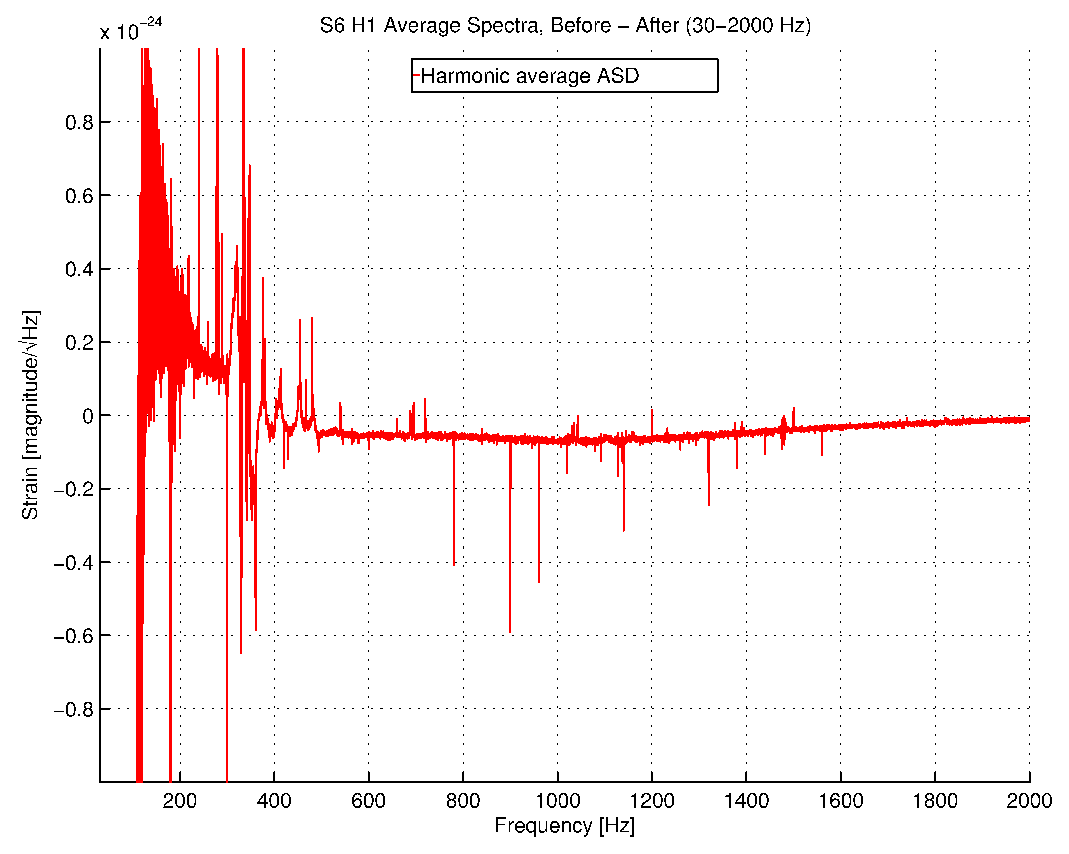
\includegraphics[height=100mm, width=75mm]{figure13a.eps}
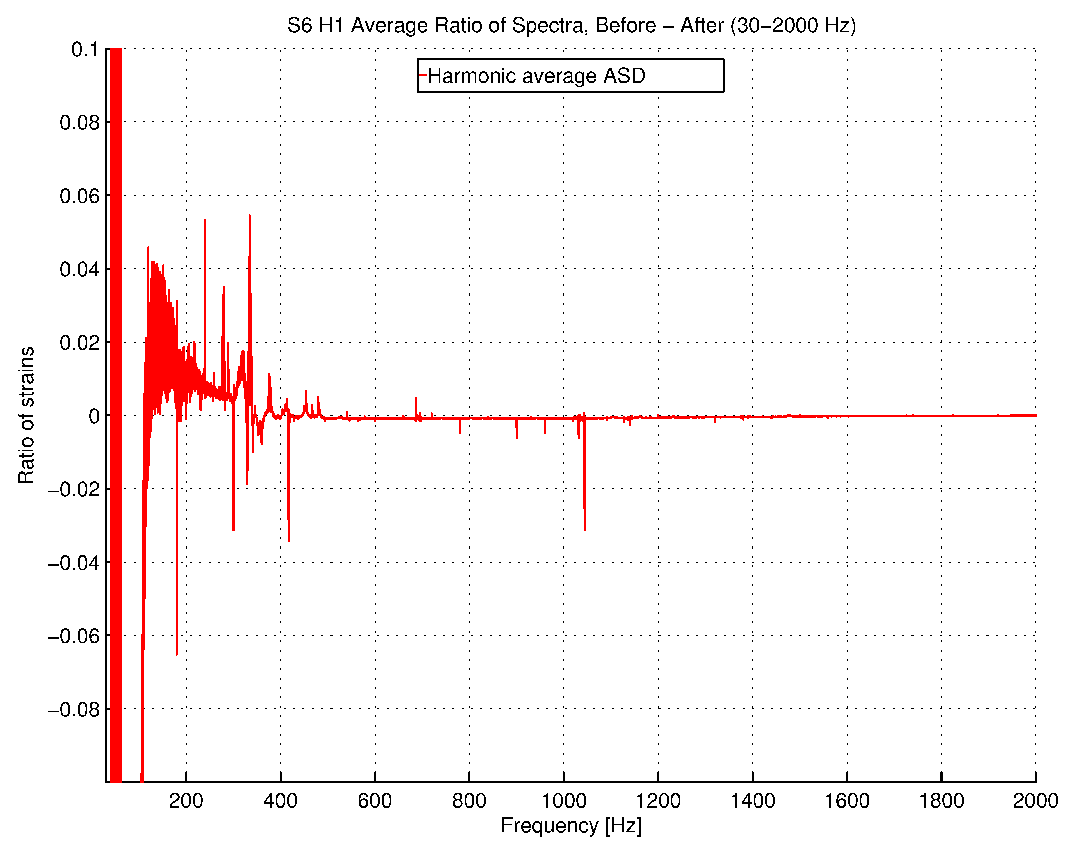
\includegraphics[height=100mm, width=75mm]{figure13b.eps}
\caption{Harmonic mean,
200 jobs from GPS second $931.0 \times 10^6$ (2009 July 07) to $932.8\times 10^6$ (2009 July 28): \textit{(before-after)} (L), \textit{(before-after)/before} (R); greater than zero is improvement.}
\label{SFTgraph}
\end{center}
\end{figure}

Note that the SFTs are high-pass filtered with a knee at 38 Hz. The harmonic mean spectrum is less susceptible to outliers than an arithmetic mean would be, and it shows a clear, several percent improvement in the band from about 80 Hz up to the violin mode frequencies. Above 400 Hz, there is slight degradation, but it is much smaller proportionally than the benefit. 

        \subsection{Feedforward benefits and potential}
        \label{benefits}

Inspiral range $\mathcal{R}$, the maximum distance at which coalescing neutron stars are likely to be detected, averaged over the sky, is one of the main LIGO figures of merit~\cite{FinnInspiral1993}. Range increases noticeably for both LIGO observatories when data from Science Run 6 is feedforward filtered; \textit{post facto} feedforward noise subtraction does improve performance. In future evolutions of this project, an explicit second-order correction for MICH-PRC coupling could yield marginally better performance. Real-time implementation and/or non-linear (frequency against frequency) methods might achieve more dramatic gains. Regardless, feedforward helps S6 sensitivity, and it should likewise help any observatory or science run with noise over a broad band due to residual contamination from auxiliary length control channels.

\begin{figure}
\begin{center}
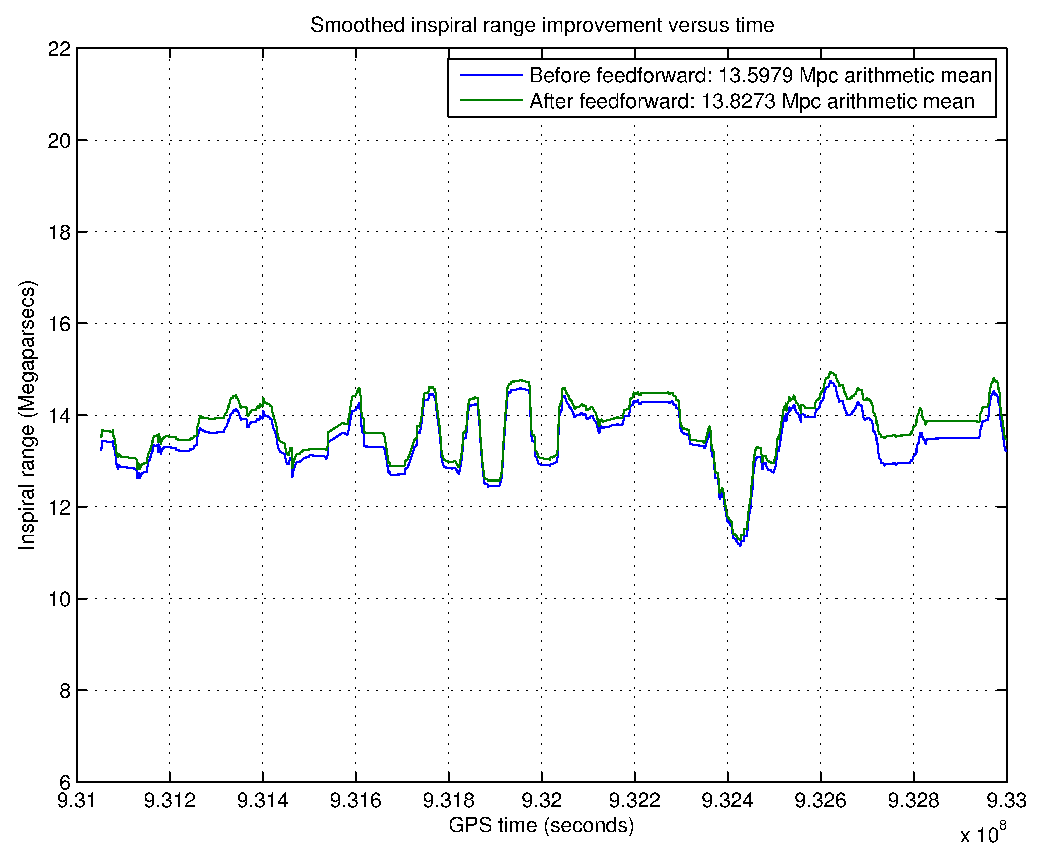
\includegraphics[height=75mm, width=150mm]{figure14a.eps}
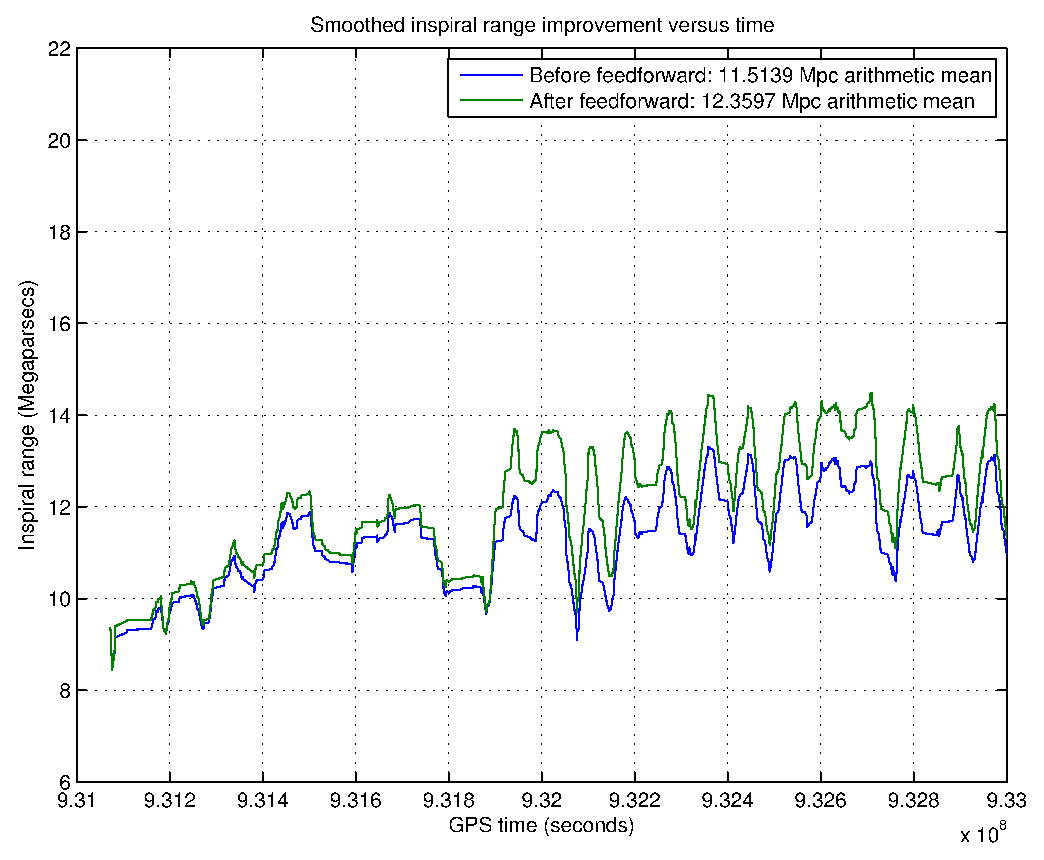
\includegraphics[height=75mm, width=150mm]{figure14b.eps}
\caption{Inspiral range vs time for Science Run 6 (starting 2009 July 07) before GPS time 9.33e8 (2009 July 30):
LIGO Hanford Observatory, H1 (top) gains 0.23 Mpc; LIGO Livingston Observatory, L1 (bottom) gains 0.84 Mpc. This graph shows the first month of S6; detector performance improved throughout the run.}
\label{S6inspiralRange}
\end{center}
\end{figure}
\begin{figure}
\begin{center}
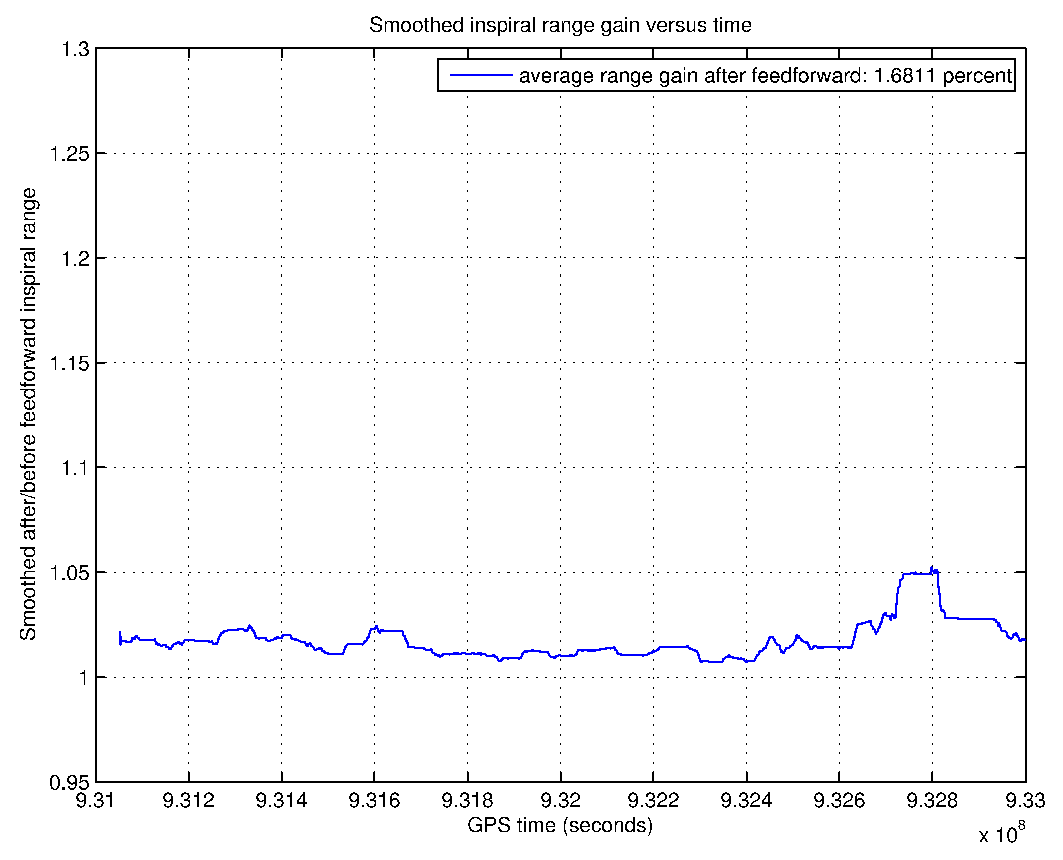
\includegraphics[height=75mm, width=150mm]{figure15a.eps}
\includegraphics[height=75mm, width=150mm]{figure15b.eps}
\caption{Inspiral range \textit{fractional gain} vs time for Science Run 6 (starting 2009 July 07) before GPS time 9.33e8 (2009 July 30):
LIGO Hanford Observatory, H1 (top) 1.68\% better; LIGO Livingston Observatory, L1 (bottom) 7.00\% better}
\label{S6inspiralRangeGain}
\end{center}
\end{figure}

From Figures~\ref{S6inspiralRange} and~\ref{S6inspiralRangeGain} we can infer the variation in the MICH and PRC couplings over a 12-day sample of S6 data. Figure~\ref{diagnosticWebpages} shows a screenshot of a webpage where LIGO data analysts can access summary graphs of the feedforward performance.

\begin{figure}
\begin{center}
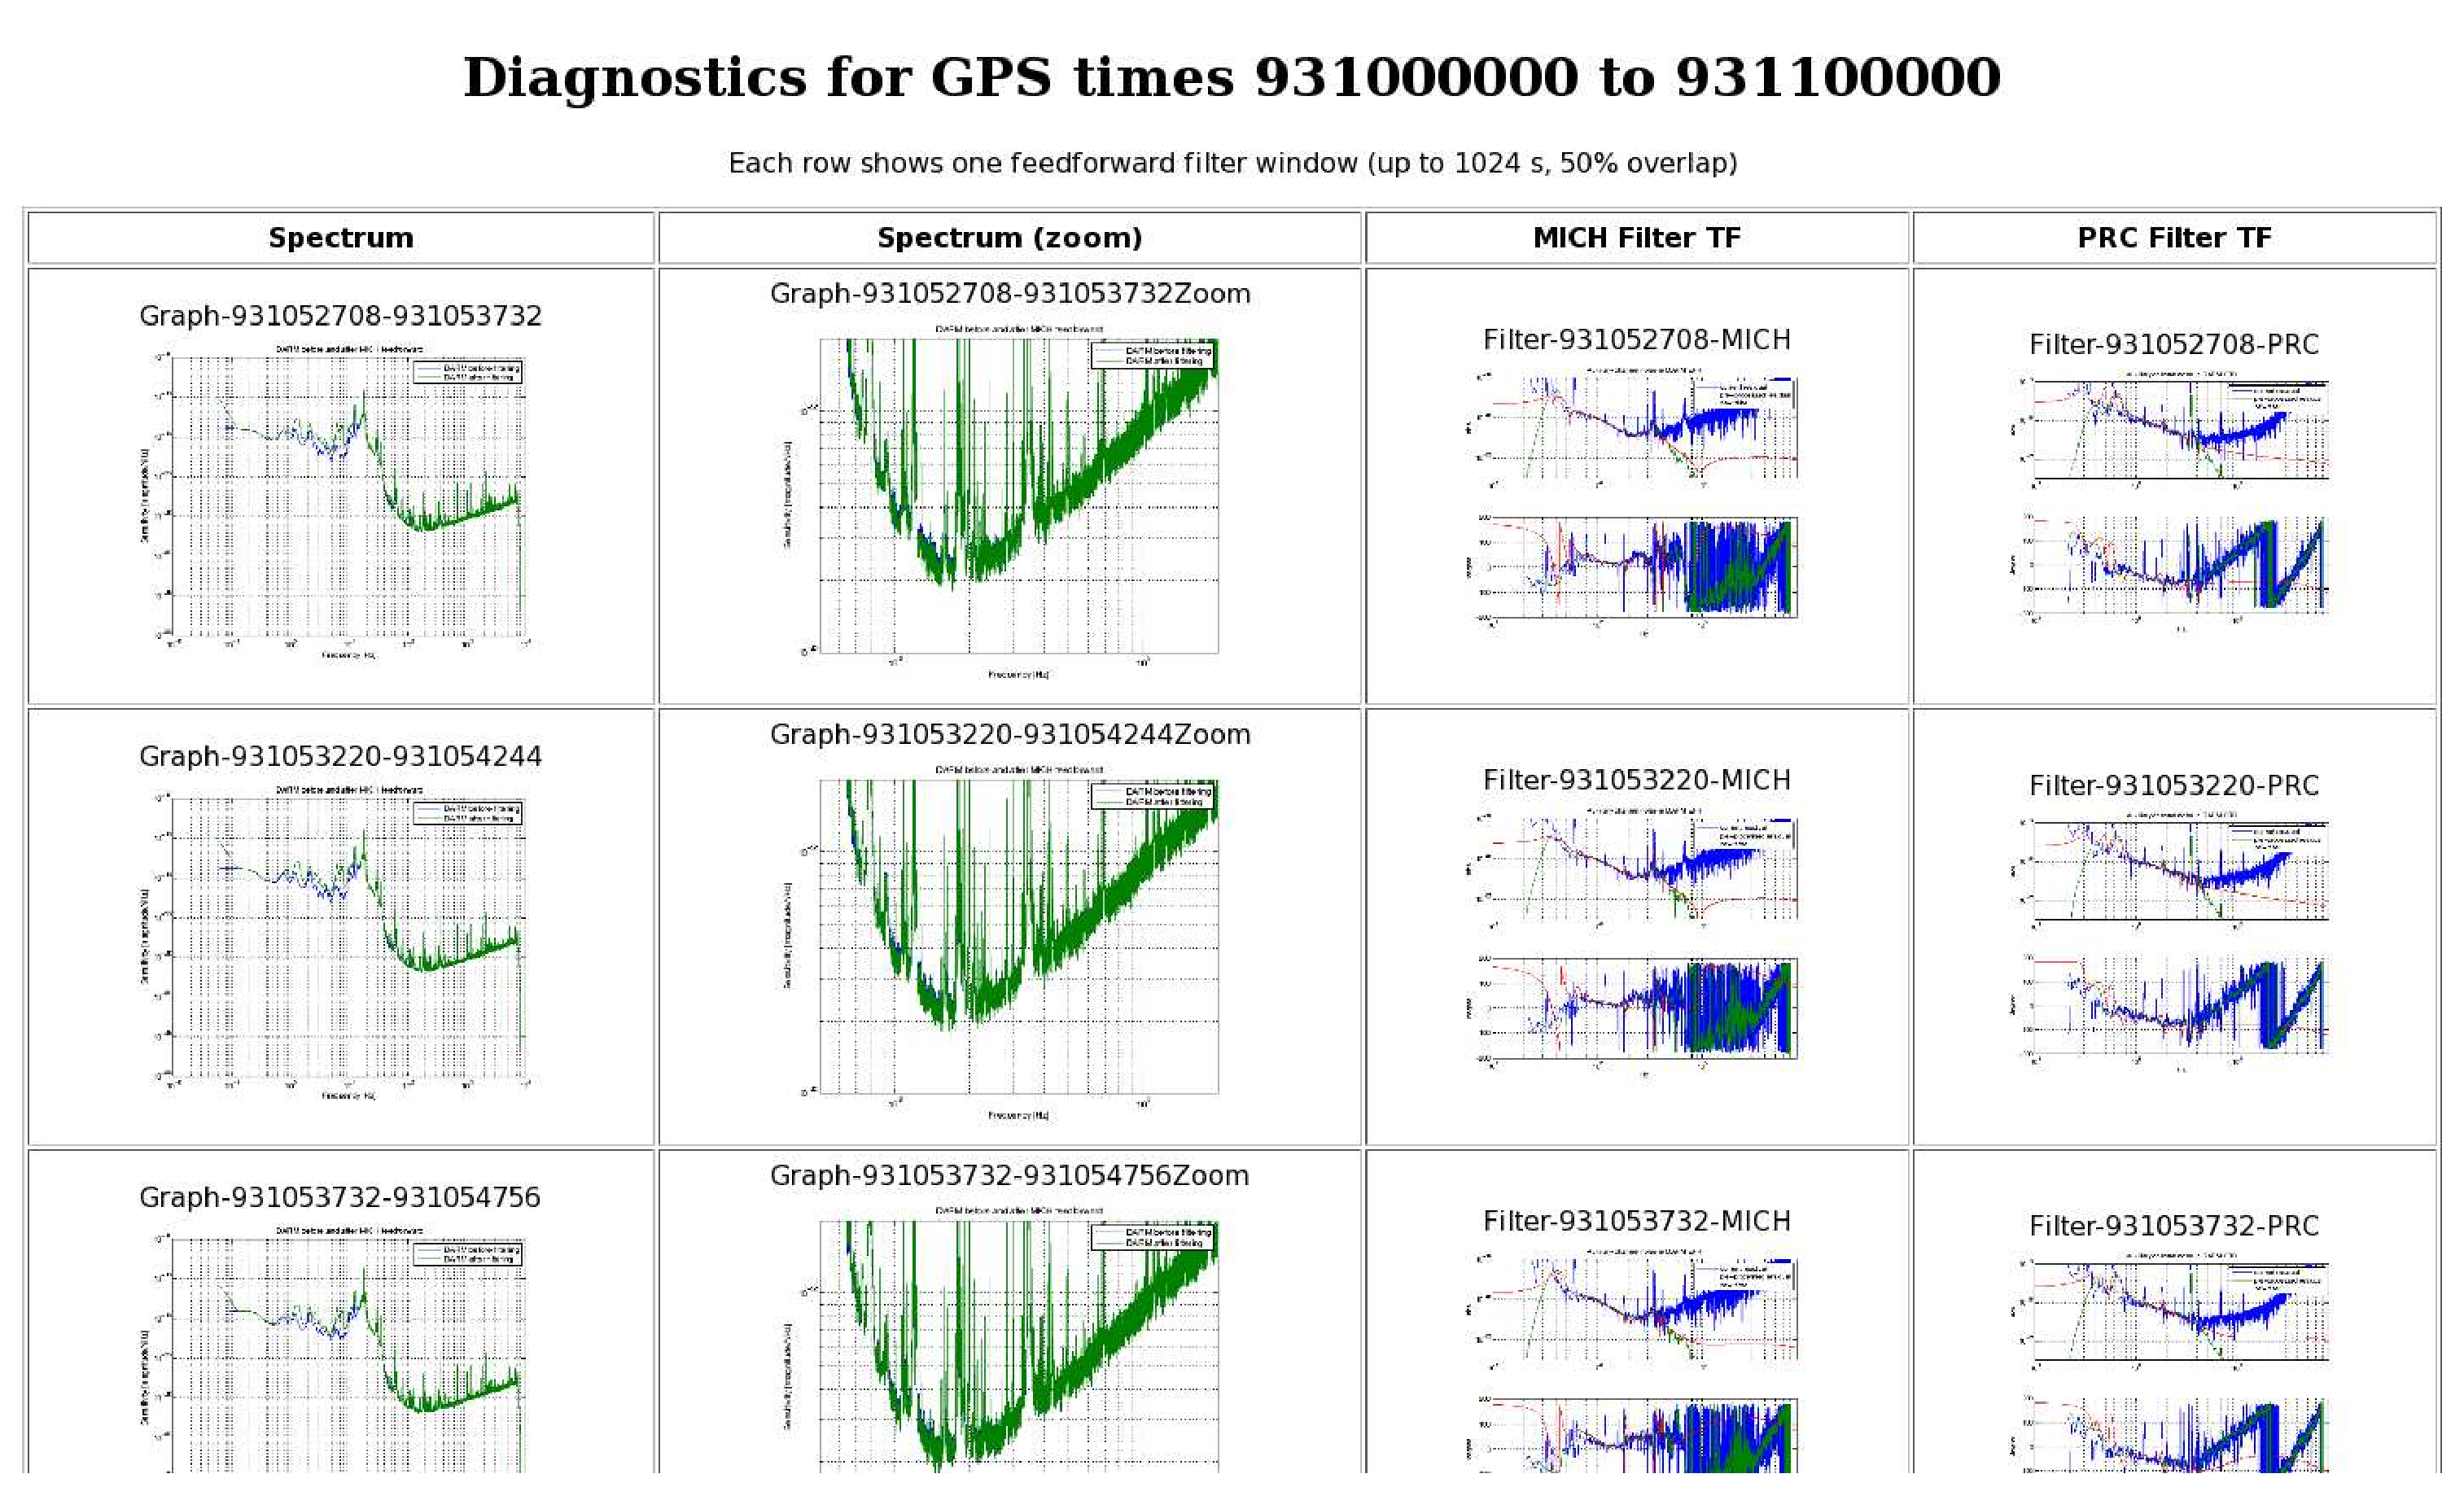
\includegraphics[height=75mm, width=150mm]{figure16.eps}
\caption{Screenshot of diagnostic web pages, indexed by window.}
\label{diagnosticWebpages}
\end{center}
\end{figure}


\section{Conclusion}

Auxiliary MICH-PRC Subtraction (AMPS) has been used to regenerate LIGO S6 data, yielding better strain sensitivity and inspiral range. Cleaned of MICH and PRC noise, data frames currently reside on the LIGO Data Grid. Frequency-domain-derived, time-domain-applied feedforward correction removes these auxiliary length control noises by fitting a rational transfer function between witness \& target. Second order sections filter the noise (witness channels), which then subtract from the measured (target) signal to yield an improved estimate of gravitational wave strain. Matlab source code can be found at the Matapps repository~\cite{MatappsRepository}. Diagnostics confirm that the corrected measurement of $h(t)$ benefits from dynamic, adaptive, algorithmic \textit{post facto} feedforward subtraction, gaining several percent in detectable inspiral range. Such an improvement potentially enhances the performance of any search using LIGO data. 

The subtraction leads to the lowest noise floor in strain sensitivity around 150 Hz of any time or interferometer so far\footnote{The highest performance to date at shot-noise limited frequencies has been obtained very differently, with quantum optical squeezing~\cite{BarsottiNatureSqueezing,DwyerPhaseNoise}}. This record may remain until Advanced LIGO begins operation. When that time comes, adaptive feedforward filters, either real-time or \textit{post facto}, can be applied to mitigate contamination from the noisy-but-inescapable parts of the tightly-coupled interferometer servo system. Signal recycling and filter cavities will only add to the complex challenge commissioning scientists face. Angular and length sensing degrees of freedom will both need finer control servos. Advanced LIGO will also contain many more physical and environmental monitors, from seismic and accelerometric to magnetic, which could provide witness channels for non-control-related noise. Altogether, many more auxiliary channels and control loops will exist in addition to MICH and PRC, and while they may require more sophisticated, non-linear methods, the subtraction technique presented here is a point of reference. Sensitive interferometry in years to come will benefit from simple yet effective methods of suppressing auxiliary instrumental influences.

LIGO was constructed by the California Institute of Technology and Massachusetts Institute of Technology with funding from the National Science Foundation and operates under cooperative agreement PHY-0757058. This paper carries LIGO Document Number LIGO-P1300193. This research was also made possible by the generous support of the National Science Foundation, awards 0855422 and 1205173, LIGO Hanford Observatory, the LIGO Scientific Collaboration, and the University of Michigan. The authors wish to thank Gregory Mendell as well as Stuart Anderson, Juan Barayoga and Dan Kozak for grid computing expertise, Ian Harry for investigating signal recovery before and after injections and providing conclusions about signal-to-noise ratio for matched filtering, and Jeff Kissel for refining MICH and PRC subtraction by hand. Tobin Fricke wrote the converter function from second-order-system to ZPK filtering and also reviewed this manuscript, as did Rana Adhikari and Jenne Driggers, who developed many of these methods at the Caltech 40 m interferometer. Michael Coughlin, Jan Harms, and Nicol\'{a}s Smith-Lefebvre all generously provided comments.

%\appendix


%\section*{References}
%\bibliographystyle{jphysicsB}
%\bibliography{Meadors_LIGO_AMPS_feedforward}
%\begin{thebibliography}
%\bibitem{book1} Goosens M, Rahtz S and Mittelbach F 1997 {\it The \LaTeX\ Graphics Companion\/} 
%(Reading, MA: Addison-Wesley)
%\bibitem{eps} Reckdahl K 1997 {\it Using Imported Graphics in \LaTeX\ } (search 
%CTAN for the file `epslatex.pdf')
%\References
%\endrefs
%\end{thebibliography}

%\end{document}

